%!TEX root = ../Thesis.tex
%% Basierend auf TeXnicCenter-Vorlage von Mark Müller
%%                      Willi Nüßer
%%                      Waldemar Penner     
%%                      Ulrich Reus
%%                      Frank Plass
%%                      Oliver Tribeß 
%%                      Daniel Hintze     
%%%%%%%%%%%%%%%%%%%%%%%%%%%%%%%%%%%%%%%%%%%%%%%%%%%%%%%%%%%%%%%%%%%%%%%

% Wählen Sie die Optionen aus, indem Sie % vor der Option entfernen  
% Dokumentation des KOMA-Script-Packets: scrguide

%%%%%%%%%%%%%%%%%%%%%%%%%%%%%%%%%%%%%%%%%%%%%%%%%%%%%%%%%%%%%%%%%%%%%%%
%% Optionen zum Layout des Artikels                                  %%
%%%%%%%%%%%%%%%%%%%%%%%%%%%%%%%%%%%%%%%%%%%%%%%%%%%%%%%%%%%%%%%%%%%%%%%
\documentclass[%
paper=A4,         % alle weiteren Papierformat einstellbar
fontsize=12pt,    % Schriftgröße (12pt, 11pt (Standard))
BCOR=12mm,         % Bindekorrektur, bspw. 1 cm
DIV=14,            % breiter Satzspiegel
parskip=half*,    % Absatzformatierung s. scrguide 3.1
headsepline,      % Trennline zum Seitenkopf  
%footsepline,     % Trennline zum Seitenfuß
%normalheadings,  % Überschriften etwas kleiner (smallheadings)
listof=totoc,     % Tabellen & Abbildungsverzeichnis ins Inhaltsverzeichnis      
%bibtotoc,        % Literaturverzeichnis im Inhalt 
%draft            % Überlangen Zeilen in Ausgabe gekennzeichnet
footinclude=false,% Fußzeile in die Satzspiegelberechnung einbeziehen 
headinclude=true, % Kopfzeile in die Satzspiegelberechnung einbeziehen 
final             % draft beschleunigt die Kompilierung
]
{scrartcl}

%\setuptoc{toc}{totoc} % Inhaltsverzeichnis ins Inhaltsverzeichnis

% Neue Deutsche Rechtschreibung und Deutsche Standardtexte
\usepackage[ngerman]{babel} 

% Umlaute können verwendet werden
\usepackage[utf8]{inputenc}   

% Echte Umlaute
\usepackage[T1]{fontenc} 

% Latin Modern Font, Type1-Schriftart für nicht-englische Texte
\usepackage{lmodern} 

% 1/2-zeiliger Zeilenabstand
\usepackage[onehalfspacing]{setspace}

% Für die Defenition eigener Kopf- und Fußzeilen
\usepackage{fancyhdr} 

% Listing Placement
\usepackage{float}

% Für die Verwendung von Grafiken
\usepackage[pdftex]{graphicx}

% Bessere Tabellen
\usepackage{tabularx}

% Für die Befehle \toprule, \midrule und \bottomrule, z.B. in Tabellen 
\usepackage{booktabs}

% Erlaubt die Benutzung von Farben
\usepackage{color}

% Verbessertes URL-Handling mit \url{http://...}
\usepackage{url}

% Listen ohne Abstände \begin{compactlist}...\end{compactlist}
\usepackage{paralist} 

% Ausgabe der aktuellen Uhrzeit für die Draft-Versionen
\usepackage{datetime}

% Deutsche Anführungszeichen
\usepackage[babel,german=quotes]{csquotes}

% Konfiguration der Abbildungs- und Tabellenbezeichnungen
\usepackage[format=hang, font={footnotesize, sf}, labelfont=bf, justification=raggedright,singlelinecheck=false]{caption}

% Verbessert die Lesbarkeit durch Mikrotypografie
\usepackage[activate={true,nocompatibility},final,tracking=true,kerning=true,spacing=true,factor=1100,stretch=10,shrink=10]{microtype}  

% Zitate und Quellenverzeichnis
\usepackage[
    bibstyle=authoryear,
    citestyle=authoryear-fhdw,  
    giveninits=false,         % false = Vornamen werden ausgeschrieben
    natbib=true,
    urldate=long,             % "besucht am" - Datum
    %url=false,
    date=long,                
    dashed=false, 
    maxcitenames=3,           % max. Anzahl Autorennamen in Zitaten
    maxbibnames=99,           % max. Anzahl Autorennamen im Quellenverzeichnis
    %backend=bibtex           % Ggf. für ältere Distributionen bibtex verwenden
    backend=biber
]{biblatex}
  
% Bibliograpthy
\bibliography{library/library}

% Keine Einrückung bei einem neuen Absatz 
\parindent 0pt 

% Ebenentiefe der Nummerierung
\setcounter{secnumdepth}{3}

% Gliederungstiefe im Inhaltsverzeichnis 
\setcounter{tocdepth}{3} 

% Tabellen- und Abbildungsverzeichnis mit Bezeichnung:
\usepackage[titles]{tocloft}

% Sourcecode-Listings
\usepackage{listings}

% Bestimmte Warnungen unterdrücken
% siehe http://tex.stackexchange.com/questions/51867/koma-warning-about-toc
% \usepackage{scrhack} % Removed to avoid missing package error

%% http://tex.stackexchange.com/questions/126839/how-to-add-a-colon-after-listing-label
\makeatletter
\begingroup\let\newcounter\@gobble\let\setcounter\@gobbletwo
  \globaldefs\@ne \let\c@loldepth\@ne
  \newlistof{listings}{lol}{\lstlistlistingname}
\endgroup
\let\l@lstlisting\l@listings
\makeatother

\renewcommand*\cftfigpresnum{Abbildung~}
\renewcommand*\cfttabpresnum{Tabelle~}
\renewcommand*\cftlistingspresnum{Listing~}
\renewcommand{\cftfigaftersnum}{:}
\renewcommand{\cfttabaftersnum}{:}
\renewcommand{\cftlistingsaftersnum}{:}
\settowidth{\cftfignumwidth}{\cftfigpresnum 99~\cftfigaftersnum}
\settowidth{\cfttabnumwidth}{\cfttabpresnum 99~\cftfigaftersnum}
\settowidth{\cftlistingsnumwidth}{\cftlistingspresnum 99~\cftfigaftersnum}
\setlength{\cfttabindent}{1.5em}
\setlength{\cftfigindent}{1.5em}
\setlength{\cftlistingsindent}{1.5em}

\renewcommand\lstlistlistingname{Listingverzeichnis}
 
% Style für Kopf- und Fußzeilenfelder
\pagestyle{fancy}
\fancyhf{}
\fancyhead[R]{\leftmark}
\fancyfoot[R]{\thepage} 
\renewcommand{\sectionmark}[1]{\markboth{#1}{#1}} 
\fancypagestyle{plain}{}

% Macro für Quellenangaben unter Abbildungen und Tabellen
\newcommand{\source}[1]{{\vspace{-1mm}\\\footnotesize\textsf{\textbf{Quelle:}} \textsf{#1}\par}}

% Anpassungen der Formatierung an Eclipse-Aussehen 
% http://jevopi.blogspot.de/2010/03/nicely-formatted-listings-in-latex-with.html
%\definecolor{sh_comment}{rgb}{0.12, 0.38, 0.18 } %adjusted, in Eclipse: {0.25, 0.42, 0.30 } = #3F6A4D
%\definecolor{sh_keyword}{rgb}{0.37, 0.08, 0.25}  % #5F1441
%\definecolor{sh_string}{rgb}{0.06, 0.10, 0.98} % #101AF9
% Für Druckausgabe sollte alles schwarz sein
\definecolor{sh_comment}{rgb}{0.0, 0.0, 0.0 }
\definecolor{sh_keyword}{rgb}{0.0, 0.0, 0.0 }
\definecolor{sh_string}{rgb}{0.0, 0.0, 0.0 }

\lstset{ %
  language=Java,
  basicstyle=\small\ttfamily,
  fontadjust, 
  xrightmargin=1mm,
  xleftmargin=5mm,
  tabsize=2,
  columns=flexible,
  showstringspaces=false,
  rulesepcolor=\color{black},
  showspaces=false,showtabs=false,tabsize=2,
  stringstyle=\color{sh_string},
  keywordstyle=\color{sh_keyword}\bfseries,
  commentstyle=\color{sh_comment}\itshape,
  captionpos=t,
  lineskip=-0.3em
}

%\makeatletter
%\def\l@lstlisting#1#2{\@dottedtocline{1}{0em}{1.5em}{\lstlistingname\space{#1}}{#2}}
%\makeatother

% Anhangsverzeichnis
\usepackage[nohints]{minitoc} %Anhangsverzeichnis

\makeatletter
\newcounter{fktnr}\setcounter{fktnr}{0}
\newcounter{subfktnr}[fktnr]\setcounter{subfktnr}{0}

\renewcommand\thesubfktnr{\arabic{fktnr}.\arabic{subfktnr}}
\newcounter{anhangcounter}
\newcommand{\blatt}{\stepcounter{anhangcounter}}

\newcommand{\anhang}[1]{\setcounter{anhangcounter}{0}\refstepcounter{fktnr}
\addcontentsline{fk}{subsection}{Anhang~\thefktnr: \hspace*{1em}#1}
\subsection*{{Anhang~\thefktnr \hspace*{1em} #1 \hspace*{-1em}}}
}

\newcommand{\subanhang}[1]{\setcounter{anhangcounter}{0}\refstepcounter{subfktnr}
\addcontentsline{fk}{subsubsection}{Anhang~\thesubfktnr: \hspace*{1em}#1}
\subsubsection*{{Anhang~\thesubfktnr \hspace*{1em} #1 \hspace*{-1em}}}
}

\newcommand{\anhangsverzeichnis}{\mtcaddsection{\subsection*{Anhangsverzeichnis \@mkboth{FKT}{FKT}}}\@starttoc{fk}\newpage}

% Links im PDF
\usepackage[pdfpagemode={UseOutlines}, plainpages=false,breaklinks=true,pdfpagelabels]{hyperref}

 % Abkürzungsverzeichnis
\usepackage[automake,
			acronym,         % create list of acronyms
            nonumberlist,
            toc, 
            section,
            nopostdot,  % avoid dot after acronym
            hyperfirst=false,% don't hyperlink first use
            %sanitize=none    % switch off sanitization as description % Deprecated
            ]{glossaries}
            \newglossarystyle{mylist}{%
\setglossarystyle{long}% base this style on the list style
\renewcommand*{\glossaryentryfield}[5]{%
    \glsentryitem{##1}\textbf{##2} & ##3 \\}%
}

% Verbessert das Referenzieren von Kapiteln, Abbildungen etc.
\usepackage[german,capitalise]{cleveref}

\makeglossaries\makeglossaries 
\input{config/Abkuerzungen.tex}


%%%%%%%%%%%%%%%%%%%%%%%%%%%%%%%%%%%%%%%%%%%%%%%%%%%%%%%%%%%%%%%%%%%%%%%
%% Parameter - Hier auf die eigene Arbeit anpassen
%%%%%%%%%%%%%%%%%%%%%%%%%%%%%%%%%%%%%%%%%%%%%%%%%%%%%%%%%%%%%%%%%%%%%%%

\newcommand{\studiengang}{Wirtschaftsinformatik} 
\newcommand{\spezialisierungsbereich}{Cyber Security}
\newcommand{\martikelnummer}{101485}
\newcommand{\dokumententyp}{Bachelorthesis}
\newcommand{\abgabedatum}{10.06.2025} 
\newcommand{\ort}{Langenfeld} 
\newcommand{\koorperationsunternehmen}{Unternehmen GmbH}
\newcommand{\fhdwstandort}{Bergisch Gladbach} % oder Bielefeld, Mettmann, ...
\newcommand{\dokumententitel}{Konzeption und Implementierung eines React-Frameworks zur flexiblen Erweiterung digitaler Datenbestände}
\newcommand{\dokumentenautor}{Thomas Benjamin Hopf}
\newcommand{\dokumentenautoradress}{Heinrichstrasse 23\\40764 Langenfeld}
\newcommand{\dokumentenpruefer}{Prof.\ Dr.\ Christian Soltenborn\\}

%%%%%%%%%%%%%%%%%%%%%%%%%%%%%%%%%%%%%%%%%%%%%%%%%%%%%%%%%%%%%%%%%%%%%%%

\hypersetup{
  colorlinks=false,
  pdfborder={0 0 0},
  pdftitle=\dokumententitel,
  pdfauthor=\dokumentenautor
} 

\begin{document}

% Römische Seitennummerierung
\pagenumbering{Roman}
 
%%%%%%%%%%%%%%%%%%%%%%%%%%%%%%%%%%%%%%%%%%%%%%%%%%%%%%%%%%%%%%%%%%%%%%%
%% Titelseite
%%%%%%%%%%%%%%%%%%%%%%%%%%%%%%%%%%%%%%%%%%%%%%%%%%%%%%%%%%%%%%%%%%%%%%%

%!TEX root = ../Thesis.tex

\begin{titlepage}

\begin{center}
\includegraphics[scale=0.8]{img/fhdw}

\vspace{7mm}

\Huge{\bfseries\dokumententyp}\\

\vspace{5mm}

\LARGE{\dokumententitel}\\

\vspace{15mm}

\large{Prüfer(in):\\

\dokumentenpruefer 

\vspace{15mm}

Verfasser(in):\\

\dokumentenautor\\

\martikelnummer\\

\vspace{3mm}

\dokumentenautoradress\\

\vspace{7mm}

\studiengang\\

\spezialisierungsbereich\\

}

\enlargethispage{2em}

\vspace{15mm}

\large{Eingereicht am:\\

\abgabedatum \\

}

\end{center}


\end{titlepage}



%%%%%%%%%%%%%%%%%%%%%%%%%%%%%%%%%%%%%%%%%%%%%%%%%%%%%%%%%%%%%%%%%%%%%%%
%% Draft-Einstellungen
%%
%% Für die finale Version auskommentieren!
%%%%%%%%%%%%%%%%%%%%%%%%%%%%%%%%%%%%%%%%%%%%%%%%%%%%%%%%%%%%%%%%%%%%%%%
\fancyhead[L]{\color{red} Stand: \today~-~\currenttime}

%%%%%%%%%%%%%%%%%%%%%%%%%%%%%%%%%%%%%%%%%%%%%%%%%%%%%%%%%%%%%%%%%%%%%%%
%% Verzeichnisse
%%%%%%%%%%%%%%%%%%%%%%%%%%%%%%%%%%%%%%%%%%%%%%%%%%%%%%%%%%%%%%%%%%%%%%%


% Sperrvermerk
\include{chapter/Sperrvermerk}

% Inhaltsverzeichnis
\tableofcontents\newpage

% Glossar
\renewcommand{\glossarypreamble}{\label{glossary}}
\printglossary[style=long, title=Glossar, toctitle=Glossar] \newpage

% Abkürzungsverzeichnis
\renewcommand{\glossarypreamble}{\label{acronyms}}
\printglossary[type=acronym, style=long, title=Abkürzungsverzeichnis, toctitle=Abkürzungsverzeichnis] \newpage

\setcounter{table}{0} % printglossary erzeugt eine Tabelle, die die Nummerierung der "echten" Tabellen durcheinander bringt.

%%%%%%%%%%%%%%%%%%%%%%%%%%%%%%%%%%%%%%%%%%%%%%%%%%%%%%%%%%%%%%%%%%%%%%%
% Verzeichnisse
%%%%%%%%%%%%%%%%%%%%%%%%%%%%%%%%%%%%%%%%%%%%%%%%%%%%%%%%%%%%%%%%%%%%%%%

% Abbildungsverzeichnis
\fancyhead[R]{\listfigurename}
\listoffigures\newpage

% Tabellenverzeichnis
\fancyhead[R]{\listtablename}
\listoftables\newpage

% Quelltextverzeichnis
\fancyhead[R]{\lstlistlistingname}
\lstlistoflistings\newpage

% Kapitelüberschriften für den Arbeitstext
\fancyhead[R]{\leftmark}

%%%%%%%%%%%%%%%%%%%%%%%%%%%%%%%%%%%%%%%%%%%%%%%%%%%%%%%%%%%%%%%%%%%%%%%
%% Inhalt
%%%%%%%%%%%%%%%%%%%%%%%%%%%%%%%%%%%%%%%%%%%%%%%%%%%%%%%%%%%%%%%%%%%%%%%

% Arabische Seitennummerierung
\pagenumbering{arabic} 

%!TEX root = ../Thesis.tex
\section{Einleitung}
Relationale Datenbanken sind weiterhin die Standardlösung für die Speicherung und Verarbeitung betrieblicher Daten in Unternehmen \footcite{Prasad2025}.  
Durch ihre rigide Struktur ermöglichen sie eine klare Trennung zwischen Datenstruktur und Anwendungsebene, wodurch eine hohe Datenintegrität sichergestellt wird \footcite{Codd1970}; \footcite{Date2003}.  
Diese rigide Struktur kann jedoch auch zu Einschränkungen führen, insbesondere wenn Tabellen zur Laufzeit erweitert werden müssten, um eine flexible und nutzerspezifische Erweiterung zu ermöglichen \footcite{Nadkarni2001}.

Auch im betrieblichen Ablauf der Bayer AG sind relationale Datenbanken mitsamt ihrer Einschränkungen allgegenwärtig.  
Dies gilt insbesondere für Abteilungen, die für Research and Development (R\&D) zuständig sind.  
Alle Projekte, die im Rahmen von Forschungsaktivitäten durchgeführt werden, werden mitsamt zusätzlicher Attribute in einer Datenbank (Newport) hinterlegt, wodurch Budgetierung und Projekt-Planung effizient und effektiv möglich ist.  
Zwar besteht die Möglichkeit, dort viele Informationen zu hinterlegen, jedoch lassen sich die vorgegebenen Spalten nicht erweitern.  
Dadurch ist es nicht möglich, benutzerspezifische Informationen, die über den Horizont von Newport hinausgehen, zu speichern und weiterzuverarbeiten.  
Um dieses Problem zu lösen, soll eine Benutzeroberfläche entwickelt werden, die diese Speicherung ermöglicht.

Im Rahmen dieser Bachelor-Arbeit soll ein flexibles technisches Framework konzipiert und umgesetzt werden, mit welchem benutzerspezifische Attribut-Erweiterungen ermöglicht werden, ohne die bestehende Datenbankstruktur der Newport-Datenbank zu verändern.  
Dabei soll untersucht werden, wie sich die eingeführte Flexibilität mit den Anforderungen an Datenintegrität und Benutzerfreundlichkeit vereinbaren lassen.

Die Arbeit gliedert sich in folgende Kapitel:  
Zuerst sollen in Kapitel 2 wichtige grundlegende Konzepte und Begriffe rund um relationale Datenbanken und flexible Datenmodellierung erläutert werden.  
Daraufhin werden die Anforderungen an das zu entwickelnde Framework sowie die Zielsetzung für das Projekt definiert.  
Die folgenden Kapitel widmen sich der technischen Konzeption und Implementierung des Front- und Backends sowie einer abschließenden Evaluation der Ergebnisse.  
Abschließend folgt ein Ausblick auf mögliche zukünftige Entwicklungen.

%!TEX root = ../Thesis.tex
\section{Grundlagen und Hintergrund}
Für die Umsetzung des Projekts ist theoretisches Wissen rund um Datenspeicherung -verarbeitung und -verteilung 
sowie Webdesign notwendig. Während grundlegendes Informatisches Fachwissen vorausgesetzt wird,
werden alle weiteren für das Verständnis dieser Arbeit relevanten Konzepte im Folgenden erläutert.
\subsection{Fixed-Schema Datenbanken}
Die Newport-Datenbank hat aufgrund ihrer großen Datenmenge und Nutzerbasis ein unveränderbares Schema.
Das bedeutet, dass die vorgegebenen Spalten nicht bearbeitet, und auch keine neuen Spalten hinzugefügt werden können.
Dadurch wird verhindert, dass die Anzahl an Spalten der Datenbank unkontrolliert wächst, was sich negativ auf Recheneffizienz
und Übersichtlichkeit auswirken könnte. \footnote{quelle bitte}
Ein Nachteil dieses Konzepts ist jedoch die geringere Flexibilität. Ohne die Möglichkeit, neue Spalten hinzuzufügen, 
sind Nutzer auf die zum Zeitpunkt der Erstellung der Datenbank vorgesehenen Informationen beschränkt.
Im Rahmen dieses Projekt soll diese Flexibilität durch Verwendung des \"Attribute-Value-Pair\"-Modells in einer umschließenden
Architektur gewährleistet werden, ohne aber die Vorteile einer Fixed-Schema Datenbank zu mindern
\subsection{Attribute-Value-Pair Modell}
Im Rahmen des Attribute-Value-Pair Modells (In Zukunft AVPM) werden Attribute, durch welche ein Objekt genauer beschrieben wird,
in eine eigenständige Tabelle ausgegliedert. Diese Tabelle ist über einen Fremdschlüssel mit dem jeweils tragenden Objekt verbunden.
Die Attribute sind in der Tabelle als Schlüssel-Wert-Paare gespeichert. Diese Struktur ermöglicht eine flexible Erweiterung der Attribute,  
ohne dass die Struktur der Datenbank verändert werden muss: \break
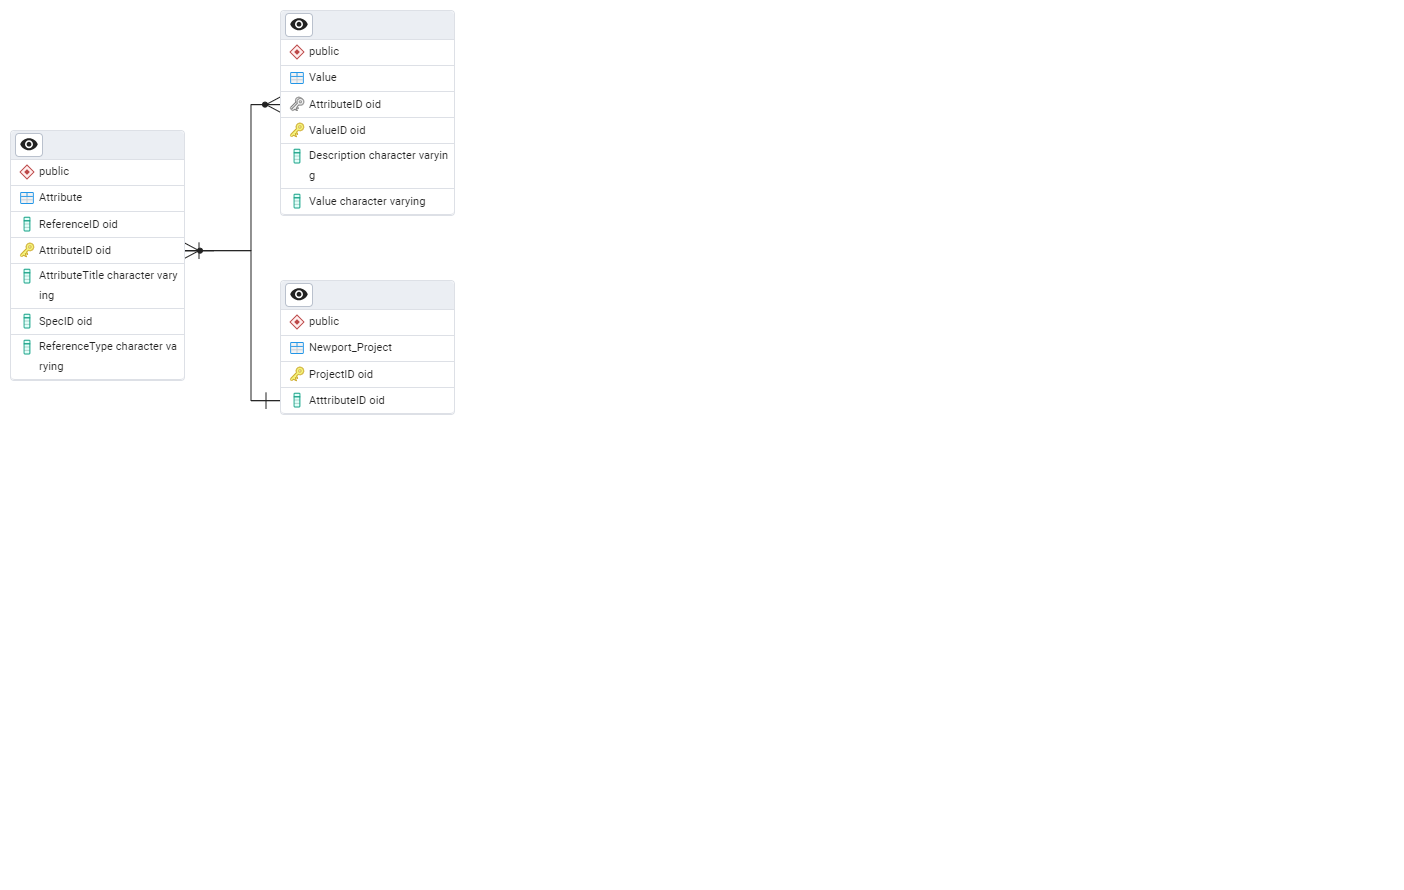
\includegraphics{C:/Bachelor/latex-thesis-template/img/avpmGraphic.png}
\subsection{Technologischer Rahmen}
Um dieses Modell im Backend umzusetzen, und dann im Front-End nutzbar zu machen, bedarf es verschiedener Technologien.
Im Backend werden die Daten in einer Aurora PostgreSQL Datenbank gespeichert\footnote{Diese Wahl beruht auf Standards im Unternehmen. Dazu mehr in der Evaluierung}. 
Aurora PostgreSQL (Im Folgenden Aurora) ist ein Dienst, der die Erstellung von relationalen Datenbanken ermöglicht. Auf dieser relationalen Datenbank ermöglicht eine 
in NodeJS \footnote{Bessere Kompatibilität mit React als alternativen} erstellte API den Zugriff auf und die Bearbeitung der gespeicherten Daten.
Auf diese API greift dann widerum eine React-App zu, die dann ermöglicht, durch eine Benutzeroberfläche die API zur Kommunikation mit der Datenbank zu benutzen.
Die Architektur ist bewusst mehrgliedrich gehalten, um Erweiterungen wie Daten-Redundanz zu ermöglichen \footnote{Unter anderem sollen die Daten in ein großes Daten
Warehouse der Bayer Cropscience kopiert werden} Die Wahl dieses technologischen Rahmens beruht auf vorhandenem Wissen und Infrastruktur im Unternehmen, sowie auch 
Abwägung der Entwicklungsgeschwindigkeit. Grundsätzlich stehen Enwticklern in der Web-Entwicklung jedoch viele Möglichkeiten zur Verfügung
\subsection{Alternative Technologien}
Für die Datenbank wäre es denkbar gewesen, anstatt einer relationalen auf eine sogenannte NoSQL Datenbanken zurückzugreifen. Eine solche Lösung
wird auch im AWS-System angeboten. Der Grund, warum sich gegen diese Option entschieden wurde, liegt in der Natur der Datengrundlage. NoSQL eignet sich vor allem für 
große Mengen unstrukturierter Daten, während traditionelle Datenbanken besser mit strukturierten Daten umgehen können \footnote{nosql source}
Im Rahmen der Anwendung muss zwingendermaßen eine strenge Typisierung von Daten gegeben sein, da auf dessen Basis unter anderem Grafiken erstellt werden sollen. 
Aus diesem Grund ist eine strukturierte Datenbank für den speziellen Zweck des Projekts besser geeignet. 
\break
Die Entscheidung, NodeJS für die API zu verwenden, beruht hauptsächlich auf der zeitlichen Komponente der Entwicklung. React basiert auf einem NodeJS-Environment, weshalb
es sich anbietet, die gleiche Umgebung für die APi zu verwenden. Grundsätzlich hätte auch jede andere Umgebung zur API-Erstellung ihren Zweck erfüllt, und diese Entscheidung 
beruht eher auf Bequemlichkeit. React hingegen als Umgebung wurde mit dem Hintergedanken der Modularität gewählt. Da das Projekt nicht nur eine einzene Anwendung, sondern eher 
einen Komplex kleinerer Tools beherbergen soll, bietet sich ein modulares Framework wie React an, wodurch dieses schon zu Beginn als Anforderung feststand, und als Basis 
aller weiteren Entscheidungen verwendet wurde. Zudem wird React unternehmensintern immer häufiger für verschiedenste Anwendungen verwendet, weshalb die Infrastruktur für das 
Deployment bereits aufgebaut ist. 

%!TEX root = ../Thesis.tex
\section{Anforderungen und Zieldefinition}
Die Anforderungen dieses Projekts gehen auf konkrete Bedürfnisse einer Nutzergruppe zurück, 
die im Arbeitsalltag intensiv mit dem System „Newport“ arbeitet. 

Im Rahmen dieser Bachelor-Arbeit soll das Minimum Viable Product (MVP) des Projekts erarbeitet werden, also 
einer ersten lauffähigen Version mit den Kernfunktionen, die von der Nutzergruppe als unverzichtbar herausgearbeitet 
wurden. Entsprechend liegt in der Anforderungskonzeptiond er Fokus auf den sogenannten "Must-Have"-Anforderungen,
ohne welche die Anwendung ihren Zweck verfehlen würde. 

Die durch interne Gespräche erfassten Nutzeranforderungen lassen sich in zwei Kategorien einteilen. An erster Stelle stehen
die funktionalen Anforderungen, die sich direkt auf die Interaktion mit der Anwendung beziehen. Ebenfalls wichtig sind jedoch auch
nicht-funktionale Anforderungen, die sich auf Qualität, Sicherheit, Performance und Wartbarkeit der Lösung beziehen.
\subsection{Funktionale Anforderungen}
\footnote{Die beiden folgenden Abschnitte dienen mehr als Platzhalter als alles anderes. Ich habe zwar schon Informationen zu den Anforderungen, werden
diese aber in den kommenden Wochen erst konkreter Ausformulieren}
Im Rahmen des Minimum Viable Products (MVP) wurden folgende funktionale Anforderungen als wesentlich identifiziert. 
Sie bilden die Grundlage für die Nutzung des Systems durch Fachanwendende ohne tiefgehendes technisches Vorwissen.
\large{1. Anlegen neuer dynamischer Attribute}\break
Nutzer*innen sollen die Möglichkeit haben, eigene Attribute anzulegen, die einem bestehenden Projektelement 
(z. B. einer Formulierung oder einem Projekt) zugewiesen werden können. Hierbei müssen folgende Angaben möglich sein:

Name des Attributs

Beschreibung (optional)

Datentyp (z. B. Text, Zahl, Datum)

\large{2. Zuweisung von Attributen zu konkreten Einträgen}\break
Bereits definierte Attribute sollen spezifischen Datenbankeinträgen zugeordnet und mit Werten befüllt werden können. Dies umfasst:

Auswahl eines vorhandenen Attributs

Eingabe eines entsprechenden Werts

Validierung des Werts entsprechend des Datentyps

\large{3. Anzeige und Bearbeitung vorhandener Attribut-Werte}\break
Im Benutzerinterface sollen alle bereits zugewiesenen Attribute mitsamt ihren Werten für ein bestimmtes Projektelement angezeigt und editierbar sein. 
Die Darstellung soll dynamisch erfolgen und sich an der Anzahl und Art der zugewiesenen Attribute orientieren.

\large{4. Löschung von Attribut-Zuweisungen}\break
Nutzer*innen sollen die Möglichkeit haben, bestehende Attribut-Wert-Paare wieder zu entfernen, ohne dabei das globale Attribut selbst zu löschen. 
Dadurch bleibt das Attribut für andere Einträge verfügbar.

\large{5. Benutzerführung und Eingabeunterstützung}\break
Die Oberfläche muss durch verständliche Beschriftungen, Platzhaltertexte, Tooltips oder andere visuelle Hinweise den Nutzer bei der Eingabe unterstützen. 
Validierungsfehler sollen unmittelbar und verständlich angezeigt werden.
\subsection{Nicht-Funktionale Anforderungen}
Neben den funktionalen Anforderungen, die die direkten Systemfähigkeiten betreffen, wurden verschiedene nicht-funktionale Anforderungen identifiziert. Diese beschreiben die Qualitätsmerkmale des Systems und sind essenziell für den erfolgreichen Betrieb in einem unternehmenskritischen Umfeld wie dem von Bayer.

\large{1. Performance}\break
Das System muss eine hohe Reaktionsgeschwindigkeit aufweisen, um eine flüssige Nutzererfahrung zu gewährleisten.

Die Ladezeit für die Anzeige eines Projektelements inklusive dynamischer Felder soll unter 500 ms liegen (bei bis zu 20 zusätzlichen Attributen).

Schreiboperationen (z. B. Hinzufügen eines Attribut-Werts) sollen ohne spürbare Verzögerung erfolgen.

\large{2. Skalierbarkeit}\break
Die Lösung soll so ausgelegt sein, dass sie mit wachsender Datenmenge und Nutzerzahl ohne grundlegende Umstrukturierung betrieben werden kann.

Die Datenbankstruktur muss große Mengen an dynamischen Attribut-Werten performant verarbeiten können.

Die Architektur (Frontend, Backend, Datenbank) muss eine horizontale Skalierung ermöglichen (z. B. API-Lastverteilung).

\large{3. Datenintegrität und Validierung}\break
Es muss sichergestellt werden, dass sämtliche gespeicherte Daten vollständig, korrekt und konsistent sind.

Alle Eingaben durch die Nutzer:innen müssen auf Plausibilität und Formatkonformität geprüft werden.

Die Datenbank muss durch Constraints und Foreign Keys inkonsistente Zustände verhindern.

\large{4. Wartbarkeit} \break
Die Codebasis soll modular und verständlich strukturiert sein, sodass zukünftige Weiterentwicklungen oder Fehlerbehebungen effizient durchgeführt werden können.

Der Quellcode muss dokumentiert sein (Kommentare, Readmes, API-Spezifikationen).

Wiederverwendbare Komponenten und Services sollen sauber gekapselt sein.

\large{5. Sicherheit} \break
Das System muss grundlegende Sicherheitsanforderungen erfüllen, um unberechtigte Zugriffe zu verhindern und sensible Daten zu schützen.

Schreibende Aktionen (z. B. das Anlegen neuer Attribute) sollen nur autorisierten Nutzern erlaubt sein.

Die API muss gegen typische Angriffe (z. B. SQL-Injection, CSRF) abgesichert sein.

Benutzerfreundlichkeit (Usability)
Die Benutzeroberfläche muss so gestaltet sein, dass auch nicht-technische Anwender:innen effektiv mit dem System arbeiten können.

Komplexe Prozesse wie das Anlegen neuer Felder sollen durch schrittweise geführte Dialoge unterstützt werden.

Fehlerzustände (z. B. ungültige Eingaben) müssen klar und verständlich kommuniziert werden.
\subsection{Abgrenzung}
Es ist zwingend notwendig, sich im Rahmen dieser Bachelorarbeit auf das MVP der Anwendung zu fokussieren, um eine abschließende
Evaluation zu gewährleisten. Dementsprechend gibt es relevante Anforderungen an das fertige Produkt, die im Rahmen dieser Bachelorarbeit 
nicht umgesetzt werden. All diese Anforderungen sollen im Folgenden der Vollständigkeit halber aufgeführt und begründet werden.\break
\large{1. Rollen-System}\break
Viele verschiedene Nutzer werden für ihre jeweiligen Vorhaben in dieser Anwendung Attribute anlegen, und diesen Werte zuweisen. Es ist durchaus denkbar,
dass zu solchen Attributen auch unter anderem geheime Daten gehören werden. Dementsprechend ist es für das finale Produkt zwingend notwendig, unbefugten Zugriff
auf eingetragene Daten zu verhindern. Dies wird über ein Rollen-System innerhalb der Datenbank geschehen, und ist in der Theorie bereits konzeptioniert. Vorerst werden
Nutzer jedoch angewiesen, keine solcher Daten zu speichern, bis dieses System fertig implementiert ist, was vorraussichtlich erst nach Ende des Bearbeitungszeitraums dieser 
Arbeit geschehen wird. Daher wird ein solches System in der Implementierung nicht beachtet.

\large{2. Internationalisierung der Oberfläche}\break
Das fertige Produkt soll, wie auch in vielen anderen Anwendungen der Fall (bspw. SAP)\footnote{quelle bitte}, in vielen verschiedenen Sprachen verfügbar sein. 
Das soll erreicht werden, indem dynamische Language Files eingesetzt werden, die auch eigens von Nutzern bereitgestellt werden können. Eine solche Implementation 
ist jedoch zeitaufwendig und aufgrund der Sprachkenntnisse der Nutzer nicht von elementarer Wichtigkeit, wird deshalb in dieser Arbeit keine Verwendung finden.\break
\large{3. Keine Integration in bestehende interne Systeme}\break
Das Projekt soll zwar publiziert werden, insbesondere um Nutzer-Rückmeldungen erhalten zu können, jedoch soll es noch nicht in die restliche IT-Landschaft integriert werden,
da das über lange Zeit und unter großer Vorsicht geschehen muss, um Kompatibilität zu garantieren.

außer diesen Anforderungen existieren mehrere Erfolgskriterien, die für das Gelingen dieses Projekts elementar wichtig sind. Diese sollen im Folgenden
herausgearbeitet werden.
\subsection{Erfolgskriterien}
In erster Linie gilt das Projekt als gescheitert, sollten die funktionalen und nicht-funktionalen Kriterien nicht erfüllt sein. 
Demnach ist es zwingend erforderlich, dass Nutzer die Anwendung zweckgemäß nutzen können, sowohl in Anbetracht der Funktionalität, als auch 
der Performanz. Um diese Kriterien in der Evaluation bewerten zu können, werden im Folgenden (soweit möglich) KPIs (Key Performance Indicators) definiert.
\subsubsection{Funktionale Zielerreichung}
Hierfür soll in erster Linie ein Abgleich zwischen den durch die Nutzer gestellten Anforderungen und der Anwendung durchgeführt werden. Die Anwendung hat
alle definierten "Must-Have"-Anforderungen zu erfüllen. Zudem sollen Nutzerinterviews geführt werden\footnote{rausstreichen wenn kb drauf}, um die Nutzerakzeptanz 
zu messen, und somit die Zweckmäßigkeit der Benutzeroberfläche zu evaluieren.
\subsubsection{Nicht-Funktionale Anforderungen}
Bei durchschnittlicher Nutzung sollte sich die Response-Time der Anwendung in verhältnismäßigen Bereichen bewegen. Diese sind unabhängig vom Endgerät des Nutzers, da es
sich um eine Cloud-Applikation handelt, und sollten 2 Sekunden nicht überschreiten \footnote{Hier ABgleich mit anderen Systemen für Vergleichbarkeit. Außerdem Gespräche mit Joerg maybe, um das herauszuarbeiten, auch it nuzern?}
\subsubsection{Zukunftstauglichkeit und Wartbarkeit}
Zusätzlich zu der imminenten Funktionalität des Programms muss gewährleistet sein, dass die Instandhaltung, sowie eventuelle Erweiterungen der Anwendung in Zukunft möglich sind.
Hierfür ist es wichtig, dass die Codebasis modular und verständlich strukturiert ist, was durch eine saubere Trennung von Frontend und Backend, sowie durch die Verwendung von Frameworks, die eine klare Struktur vorgeben erreicht wird.
Über diese Arbeit hinaus muss demnach eine Dokumentation gegeben sein, mitdessen Hilfe der Code der Anwendung verständlich ist.



%!TEX root = ../Thesis.tex
\section{Systemdesign und Herausforderungen}
Die Architektur ist im Sinne der Übersicht und Erweiterbarkeit klar in drei Teile aufgeteilt. 
Zur Datenspeicherung wird eine Aurora-Datenbank verwendet, mit welcher über eine NodeJS API von einem in 
React erstellten User Interface kommuniziert werden kann. Die Datenbank soll in der Lage sein, 
Attribut-Wert-Paare flexibel beherbergen zu können, und dabei die bestmögliche Performanz aufweisen.
\subsection{Datenbankarchitektur}
Um die Erweiterbarkeit der Anwendung zu garantieren, muss die Datenstruktur fest sein. \footnote{quelle bitte} Trotzdem muss die Datenbank aber 
in der Lage sein, flexibel unterschiedliche Attribute und Werte speichern zu können. Das soll folgende Datenstruktur erreichen:\break

\begin{figure}[hbt]
    \centering
    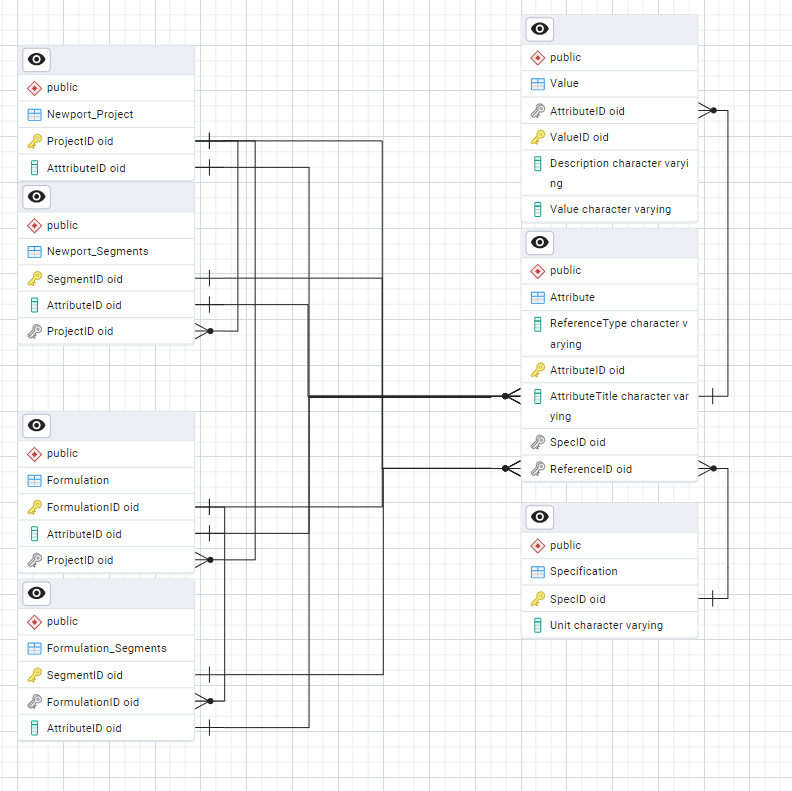
\includegraphics[width=\textwidth]{C:/Bachelor/latex-thesis-template/img/datenstruktur.png} 
    \caption{Modell der Datenbank}
    \label{fig:deinbild}
\end{figure}
Die Datentruktur lässt sich in drei wesentliche Schichten aufteilen: An erster Stelle stehen die festen Datenobjekte, 
welche gleichlautend aus der bestehenden Infrastruktur übernommen werden. Diese Schicht bildet das Bindeglied zwischen der bereits existierenden Datenlandschaft 
und der von dieser Anwendung angehängten flexiblen Daten. Darauf folgt die dynamische Attributzuordnung, die über Fremdschlüssel direkt mit der ersten Schicht verbunden ist.
Sie dient zur Verlinkung verschiedener Attribute mit ihren jeweiligen Eltern-Tabellen, speichert zusätzlich aber auch grundlegende Informationen über die Attribute ab. 
Die dritte Schicht beherbergt die Werte, und verbindet diese mit ihren zugehörigen Attributen. In dieser Schicht sind Informationen zu der Natur der Werte, aber auch zum Inhalt abgespeichert. 
Im Folgenden sollen diese drei Schichten mir ihren jeweiligen Tabellen genauer beleuchtet werden. 
\subsubsection{Schicht 1 Domänenspezifische Tabellen}
\enquote{Newport\_Project} bildet das übergeordnete Forschungsprojekt und ihre zugehörigen Daten ab, wobei \"Formulation\" nur ein Forschungsobjekt beschreibt, welches an ein Projekt geknüpft sein kann,
aber nicht unbedingt muss: 


\begin{table}[hbt]
    \centering
    \caption{Newport\_Project}
    \begin{tabularx}{\textwidth}{l l l X}
        \toprule
        \textbf{Spalte} & \textbf{Datentyp} & \textbf{Schlüssel?} & \textbf{Beschreibung} \\
        \midrule
        ProjectID & Object Identifier (oid) & Primärschlüssel & Primärer Identifier für den Eintrag \\
        AttributeID & Object Identifier (oid) & Fremdschlüssel & Verweis auf zugewiesene Attribute für das jeweilige Projekt \\
        \bottomrule
    \end{tabularx}
    \source{Eigene Darstellung}
    \label{tab:newport_project}
\end{table}

\begin{table}[hbt]
    \centering
    \caption{Formulation}
    \begin{tabularx}{\textwidth}{l l l X}
        \toprule
        \textbf{Spalte} & \textbf{Datentyp} & \textbf{Schlüssel?} & \textbf{Beschreibung} \\
        \midrule
        FormulationID & Object Identifier (oid) & Primärschlüssel & Primärer Identifier für den Eintrag\\
        AttributeID & Object Identifier (oid) & Fremdschlüssel & Verweis auf zugewiesene Attribute für das jeweilige Projekt\\
        ProjectID & Object Identifier (oid) & Fremdschlüssel & Verweis auf ein gegebenenfalls zugewiesenes Newport-Projekt\\
        \bottomrule
    \end{tabularx}
    \source{Eigene Darstellung}
    \label{tab:formulation}
\end{table}

\begin{table}[hbt]
    \centering
    \caption{Newport\_Segments}
    \begin{tabularx}{\textwidth}{l l l X}
        \toprule
        \textbf{Spalte} & \textbf{Datentyp} & \textbf{Schlüssel?} & \textbf{Beschreibung} \\
        \midrule
        SegmentID & Object Identifier (oid) & Primärschlüssel & Primärer Identifier für den Eintrag\\
        AttributeID & Object Identifier (oid) & Fremdschlüssel & Verweis auf zugewiesene Attribute für das jeweilige Segment\\
        ProjectID & Object Identifier (oid) & Fremdschlüssel & Verweis auf das zugehörige Newport-Projekt\\
        \bottomrule
    \end{tabularx}
    \source{Eigene Darstellung}
    \label{tab:formulation}
\end{table}

\begin{table}[hbt]
    \centering
    \caption{Formulation\_Segments}
    \begin{tabularx}{\textwidth}{l l l X}
        \toprule
        \textbf{Spalte} & \textbf{Datentyp} & \textbf{Schlüssel?} & \textbf{Beschreibung} \\
        \midrule
        SegmentID & Object Identifier (oid) & Primärschlüssel & Primärer Identifier für den Eintrag\\
        Formulation & Object Identifier (oid) & Fremdschlüssel & Verweis auf zugewiesene Attribute für das jeweilige Segment\\
        ProjectID & Object Identifier (oid) & Fremdschlüssel & Verweis auf das zugehörige Newport-Projekt\\
        \bottomrule
    \end{tabularx}
    \source{Eigene Darstellung}
    \label{tab:formulation}
\end{table}

\begin{table}[hbt]
    \centering
    \caption{Attribute}
    \begin{tabularx}{\textwidth}{l l l X}
        \toprule
        \textbf{Spalte} & \textbf{Datentyp} & \textbf{Schlüssel?} & \textbf{Beschreibung} \\
        \midrule
        ReferenceType & String (oid) & / & Automatisch gesetzte wörtliche Referenz auf den Owner des Attributs\\
        ReferenceID & Object Identifier (oid) & Fremdschlüssel & Direkter Verweis auf den Owner des Attributs\\
        AttributeID & Object Identifier (oid) & Primärschlüssel & Verweis auf das zugehörige Attribut\\
        AttributeTitle & String & / & Titel des Attributs\\
        SpecID & Object Identifier (oid) & Fremdschlüssel & Verweis auf die zugehörige Spezifikation\\
        \bottomrule
    \end{tabularx}
    \source{Eigene Darstellung}
    \label{tab:formulation}
\end{table}

\begin{table}[hbt]
    \centering
    \caption{Value}
    \begin{tabularx}{\textwidth}{l l l X}
        \toprule
        \textbf{Spalte} & \textbf{Datentyp} & \textbf{Schlüssel?} & \textbf{Beschreibung} \\
        \midrule
        AttributeID & Object Identifier (oid) & Fremdschlüssel & Verweis auf das zugehörige Attribut\\
        ValueID & Object Identifier (oid) & Primärschlüssel & Primärer Identifier für den Eintrag\\
        Description & String & / & Name des Werts\\
        Value & String & / & Wert\\
        \bottomrule
    \end{tabularx}
    \source{Eigene Darstellung}
    \label{tab:formulation}
\end{table}

\begin{table}[hbt]
    \centering
    \caption{Specification}
    \begin{tabularx}{\textwidth}{l l l X}
        \toprule
        \textbf{Spalte} & \textbf{Datentyp} & \textbf{Schlüssel?} & \textbf{Beschreibung} \\
        \midrule
        SpecID & Object Identifier (oid) & Primärschlüssel & Primärer Identifier für den Eintrag\\
        Unit & String & / & Einheit\\
        \bottomrule
    \end{tabularx}
    \source{Eigene Darstellung}
    \label{tab:formulation}
\end{table}

\subsection{Herausforderungen}
Im Folgenden sollen die Herausforderungen, die die Anforderungen an das Projekt posieren, und mögliche Lösungsansätze für diese diskutiert
werden. 
\subsubsection{Datenkonsistenz}
Aufgrund der hohen Flexibilität der einzutragenen Daten muss die Datenbank modular aufgebaut sein. Um die Datenkonsistenz zu garantieren, 
muss aber verhindert werden, dass durch die API (Direkte Manipulation ist in der Architektur nicht vorgesehen) inkorrekte Daten in die Datenbank
eingespeist werden. Dafür müssen alle API-Requests noch vor Absendung auf Validität geprüft werden. Schlägt die Prüfung an, soll der Nutzer über den 
Fehler inkenntnis gesetzt werden. Da die Datenbank modular aufgebaut ist, muss die Erweitbarkeit und Performanz sichergestellt werden.
\subsubsection{Erweiterbarkeit und Performanz}
Um die Erweiterbarkeit zu garantieren, speichert die Datenbank auch Informationen, die im momentanten Scope noch nicht zwingend Erforderlich sind,
jedoch bei eventuell auftretenden Erweiterungen notwendig werden können. Ein Beispiel dafür ist die Tabelle \enquote{Specification}. Sie speichert genauere Informationen
über die Eigenschaften der Werte wie der Einheit ab. Das ist noch nicht erforderlich, da alle vorhersehbaren Daten Numerisch sind, sobald sich das aber ändert kann 
die Erweiterung ablaufen, ohne die Datenbank-Struktur zu verändern, was wichtig ist, da für eine solche Veränderung das gesamte Backend umgeschrieben werden muss. Es ist 
effizienter, die möglichen Veränderungen sofort einzuplanen. Dabei darf die Performanz aber nicht vernachlässigt werden. Durch die vielen Sicherheitsmechanismen, hinter welchen
die Daten auf AWS gelagert werden wird die Response-Time ohnehin verlängert, der restliche Prozess muss sich daran also anpassen. Der Nutzer soll jederzeit über den Fortschritt
ausstehender Anfragen informiert werden, die Anwendung muss, auch während einer laufenden Anfrage, weiter bedienbar sein und alle Prozesse rund um den Datenabruf müssen 
optimiert sein. Ein Beispiel für eine optimierende Planung in der Architektur ist die Spalte \enquote{ReferenceType}. Durch diese Spalte, die automatisch gesetzt wird, müssen die großen
Tabellen von Attribut und Attribut-Owner nicht miteinander verbunden werden, um sie zuzuordnen, wodurch (bei größeren Datenmengen in den Tabellen) die Response Time deutlich verbessert wird.
Trotz dieser Optimierungen darf aber die Architektur nicht so komplex werden, dass die Wartbarkeit darunter leidet.
\subsubsection{Wartbarkeit und Benutzerfreundlichkeit}
Die Gesamtarchitektur muss stets, trotz aller Herausforderungen, simpel genug sein, um mit möglichst geringem zusätzlichen Arbeitsaufwand gepflegt werden zu können.
Dementsprechend muss die Gesamtheit der Architektur bis ins Detail dokumentiert, und alle Entscheidungen festgehalten werden. Neben den Entwicklern, die für die Wartung zuständig sind, 
müssen aber auch die Nutzer in der Lage sein, die Anwendung zu verstehen und effektiv anzuwenden. Deshalb muss das User Interface so selbsterlklärend wir möglich sein, und alles weitere 
in einer User-Dokumentation festgehalten werden, auf welche auch offensichtlich genug verwiesen wird. 
 


%!TEX root = ../Thesis.tex
\section{Datenmodellierung}
Im Sinne der Modularität basiert die Datenmodellierung auf dem Entity-Value-Attribut-Konzept (EAV). Dieses Konzept ermöglicht die Erweiterung 
des starren relationalen Schema um eine variable Anzahl benutzerdefinierter Attribute, ohne dabei eine Schema-Veränderung zu erfordern. Dadurch 
sind die dynamischen Attribute von den Domänenobjekten (Projekte und Formulationen) getrennt. Im Folgenden soll der Aufbau und die Funktionsweise
des Datenmodells genauer erläutert werden.
\subsection{ER-Modell und Tabellenübersicht}
Das relationale Schema gliedert sich in 3 Hauptblöcke: Domänentabellen, Attributdefinition und der Werteebene. 
\subsubsection{Domänentabellen}
\enquote{Newport\_Project} verbindet die Datenbank über den Primärschlüssel \enquote{ProjectID} mit der Newport-Datenbank aus dem CropScience Warehouse (CSW). 
Das ermöglicht indirekten Zugriff auf externe Projektdaten. \enquote{Newport\_Segments} beinhaltet sogenannte Segmente\footnote{Segmente sind in der Enwticklung einer Formulation beispielsweise verschiedene Länder, in denen das Produkt lizensiert werden soll} 
für die jeweiligen Newport-Projekte, und (sofern gegeben) deren Attribute. \enquote{Formulation} und \enquote{Formulation\_Segments} fungieren entsprechend für 
zu speichernde Formulationen.
\subsubsection{Attributdefinition}
\enquote{Attribute} enthält alle potentiell verwendbaren, dynamischen Felder. Jede Zeile verfügt über eine eindeutige \enquote{AttributeID}, einen entsprechenden \enquote{AttributeTitle},
und sowohl eine direkte (\enquote{ReferenceType}), als auch eine indirekte Referenz(\enquote{ReferenceID}) auf den Attribut-Owner. Mit der \enquote{SpecID} wird zusätzlich
auf eine Tabelle verwiesen, in der genauere Informationen über das Attribut (bspw. Einheit) hinterlegt werden können.
\subsubsection{Werteebene}
\enquote{Value} speichert die benutzerdefinierten Werte, mit denen das Attribut angelegt wurde. Wesentliche Spalten sind \enquote{ValueID}, der Primärschlüssel, \enquote{AttributeID},
die Referenz auf das zugehörige Attribut, \enquote{Description} für eine mögliche genauere Beschreibung und \enquote{Value}, worin der eigentliche Wert gespeichert wird.
\subsection{Beziehungen und Referentialität}
Ein Domänenobjekt kann über die AttributeID mit beliebig vielen Attributen verbunden werden. Ein Attribut kann widerum nur einem Domänenobjekt zugewiesen werden. 
Die referentielle Integrität wird durch die Fremdschlüssel-Paarungen sichergestellt, wonach kein Attribut ohne Verweis auf ein Domänenobjekt erstellt werden kann. 
Die API ist hingegen dafür zuständig, dass ein Attribut nicht auf mehrere verschiedene Domänenobjekte verweist, indem es benutzerdefiniertes Setzen der AttributeID verhindert.
\subsection{Datenkonsistenz und Validierung}
Das EAV-Modell sieht vor, dass die Datenintegrität durch die mit der Datenbank verbundene API sichergestellt wird, indem eingegebene Werte stets auf Validität geprüft werden.
Folgende Prüfungen sind für die API vorgesehen:
\subsubsection{Datentypprüfung}
Jedes Attribut hat in der Specification einen hinterlegten Datentyp. Sollte der vom Benutzer angegebene Datentyp nicht in der Menge unterstützter Datentypen vorhanden sein,
soll die Erstellung des Attributs verhindert werden und eine entsprechende Fehlermeldung ausgegeben.
\subsubsection{Pflichtfelder und Standardwerte}
Um eine reibungslose Behandlung fehlerhafter Nutzerangaben sicherzustellen, soll schon das Front-End Pflichtfelder als solche markieren, und das Abschicken der Form verhindern,
bis diese ausgefüllt sind. Das Setzen der Schlüssel übernimmt jedoch das Backend, weshalb diese, obwohl sie Pflichtfelder sind, nicht vom Nutzer gesetzt werden müssen.
\subsubsection{Transaktionen}
Das Anlegen eines neuen Attributs und das direkte Zuweisen eines ersten Werts sollen in einer Transaktion gebündelt sein, um zu verhindern, dass Attribute ohen zugehörige Werte 
existieren.
\subsection{Beispielhafte Speicherung}
Angenommen, ein Nutzer legt für \enquote{Projekt A} ein neues Attribut \enquote{Versuchsdauer} (Einheit Integer) an und vergibt den Wert \enquote{3},
dann sähen die Abläufe und Datenbankeinträge folgendermaßen aus:
\begin{table}[h]
    \centering
    \caption{Attributdefinition}
    \label{tab:attribute}
    \begin{tabular}{@{}cccc@{}}
        \toprule
        \textbf{AttributeID} & \textbf{AttributeTitle} & \textbf{ReferenceType} & \textbf{SpecID} \\ 
        \midrule
        42 & Versuchsdauer & Newport\_Project & 2 \\ 
        \bottomrule
    \end{tabular}
\end{table}
\begin{table}[h]
    \centering
    \caption{Specification (Einheitenzuordnung)}
    \label{tab:specification}
    \begin{tabular}{@{}cc@{}}
        \toprule
        \textbf{SpecID} & \textbf{Unit} \\ 
        \midrule
        2 & Integer \\ 
        \bottomrule
    \end{tabular}
\end{table}
\begin{table}[h]
    \centering
    \caption{Speicherung eines Attribut-Wert-Paares}
    \label{tab:value}
    \begin{tabular}{@{}ccccc@{}}
        \toprule
        \textbf{ValueID} & \textbf{AttributeID} & \textbf{Description} & \textbf{Value} \\ 
        \midrule
        101 & 42 & null & 3 \\ 
        \bottomrule
    \end{tabular}
\end{table}

Durch diese Trennung bleiben das feste Schema in \enquote{Newport\_Project} und die dynamischen Erweiterungen 
klar voneinander getrennt, und trotzdem werden alle zusätzlichen relevanten Informationen abgespeichert.

Mit diesem Datenmodell können beliebig viele neue Attribute hinzugefügt werden, ohne das Grundschema der Domänentabelle anzupassen.

%!TEX root = ../Thesis.tex
\section{Bakend-Implementierung}
Im Backend übernimmt eine mit Node.js implementierte API die Geschäftslogik. Da die Daten in AWS hinter einer Firewall liegen,
sitzt die API in einer EC2-Instanz, die eine Schnittstelle zwischen der gesicherten AWS-Landschaft und externen Apps bildet. 
Zustäzlich wird API Gateway, ein AWS-Serice verwendet, um den automatisierten Zugriff auf die API zu ermöglichen. Gespeichert sind 
die Daten in einer Aurora PostgreSQL Datenbank. 
\subsection{Datenbank}
Zur Implementierung der Datenbank auf der EC2-Instanz muss zuerst eine Verbindung mit derlokalen Datenbankmanagement-System aufgebaut werden.
Dafür wird die AWS-CLI verwendet.\footnote{https://aws.amazon.com/cli/} Mit ihr wird dann\footnote{Nach Authentifizierung mit aws login --\{user\}} 
ein Tunnel zwischen dem lokalen Port 2222\footnote{Der Port ist frei wählbar, solange er nicht reserviert ist (bspw. 22 ist nicht wählbar, da belegt durch TCP)} und
dem TCP-Port 22 der EC2-Instanz geöffnet:
\begin{figure}[bht]
    \begin{lstlisting}[caption=SSH-Tunnel mit AWS-CLI, label=list:tunnel]
        aws  --profile {Profile-ID} ec2-instance-connect open-tunnel --instance-id {Instance ID} --remote-port 22 --local-port 2222 --region eu-central-1
    \end{lstlisting}
    %\footnoterule{}
    %\footnotesize{Casts have been omitted for the sake of readability}
\end{figure}
Dieser Tunnel ist zwingend erforderlich, da aufgrund von Sicherheitsrichtlinien Bayer's die EC2-Instanz keine öffentliche IP haben darf.\\
In PgAdmin kann nun eine Verbindung zu der Datenbank hergestellt werden. Dafür werden folgende Informationen benötigt:
\begin{compactenum}
	\item Host name/Adresse: Die URL der Datenbank auf AWS-Ebene (name.id.server.rds.amazonaws.com)
	\item Port: 5432 (Standard Postgres-Port)
	\item Maintenaince Database: Name der Datenbank auf AWS
	\item UserName: Name des Nutzers, mit dem auf die Datenbank zugegriffen werden soll
	\item Parameter \enquote{SSL Mode}: \enquote{prefer}
	\item Use SSH Tunneling: \enquote{enabled}
	\item Tunnel Host: localhost (da der SSH-Tunnel auf dem localhost aufgesetzt ist)
	\item Tunnel Port: 2222 (entspricht --local-port in der CLI)
	\item Authentication: \enquote{Identity File}
	\item Identity File: Hier das .pem-File hinterlegen\footnote{Key-Files können im AWS-Dashboard unter EC2 erstellt werden}
\end{compactenum}

Mit diesen Einstellungen kann der Server gespeichert werden, und ein Zugriff auf die Datenbank ist möglich. In PgAdmin kann nun wie üblich das 
geplante Schema umgesetzt werden. Nun müssen die Daten in React abrufbar gemacht werden.

\subsection{API}
Für die API muss zuerst eine Infrastruktur in AWS errichtet werden, die eine sichere Verbindung zwischen AWS-Externen Clients und den AWS-Internen
Daten garantieren kann. Diese Infrastruktur sieht folgendermaßen aus:
(Hier bild)
An erster Stelle steht die Virtual Private Cloud (VPC). Auf ihr liegt die gesamte Infrastruktur. Inbound und Outbound traffic aller IP-Adressen sind vollständig
blockiert, um die Sicherheit der Daten zu gewährleisten. Auf dieser VPC liegt die Datenbank, auf welche Zugriff durch eine EC2-Instanz ermöglicht wird. 
Die Datenbank ist eine Aurora Postgres Datenbank in Standardausführung\footnote{Standardausführung festgelegt durch den Unternehmensinternen Softwarekatalog}. Die EC2-Instanz
entspricht ebenfalls der Standardausführung, und ist so eingerichtet, dass Inbound-traffic auf TCP-Ebene ausgehend von AWS-Internen IP-Adressen möglich ist.
Zusätzlich ist die EC2-Instanz mit einem Network Load Balancer (NLB) ausgestattet, wodurch andere AWS-Programme direkt auf Elemente innerhalb der VPC zugreifen können. Dieser Zugriff ist
durch eine Target Group möglich, über den ein NLB standardmäßig verfügt, und welcher in diesem Fall direkt auf das VPC zeigt. 
In einem NodeJS-Programm, welches direkt auf der EC2-Instanz liegt, wird eine Proxy errichtet, mit der eine Verbindung nach außen hergestellt wird:
\begin{figure}[bht]
    \begin{lstlisting}[caption=EC2-Proxy in NodeJS, label=list:proxy]
        // Load .env at startup
		require('dotenv').config();

		const express = require('express');
		const morgan = require('morgan');
		const { Pool } = require('pg');

		// Sanitize and trim environment variables
		const dbUser = process.env.DATABASE_USER?.trim();
		const dbPass = process.env.DATABASE_PASSWORD?.trim();
		const dbHost = process.env.DATABASE_HOST?.trim();
		const dbPort = Number(process.env.DATABASE_PORT);
		const dbName = process.env.DATABASE_NAME?.trim();

		console.log('Starting DB proxy service');
		console.log('CWD:', process.cwd());
		console.log('Database config:', { host: dbHost, port: dbPort, user: dbUser, database: dbName });

		// Set up Express
		const app = express();

		// 1. Morgan for HTTP logging
		app.use(morgan(':method :url :status :res[content-length] - :response-time ms'));

		// 2. JSON body parsing
		app.use(express.json());

		// 3. Sanity dump for POST bodies
		app.use((req, res, next) => {
		if (['POST','PUT','PATCH'].includes(req.method)) console.log('> BODY:', req.body);
		next();
		});

		// 4. Postgres pool using sanitized env
		const pool = new Pool({
		host: dbHost,
		port: dbPort,
		user: dbUser,
		password: dbPass,
		database: dbName, 
		ssl: { rejectUnauthorized: false }
		});

		// Async wrapper helper
		defaultWrapAsync = fn => (req, res, next) => fn(req, res, next).catch(next);

		// 5. Health endpoint
		defaultWrapAsync(async (req, res) => {
		await pool.query('SELECT 1');
		res.sendStatus(200);
		});
		app.get('/health', defaultWrapAsync(async (req, res) => res.sendStatus(200)));

		// 6. Query endpoint
		app.post('/query', defaultWrapAsync(async (req, res) => {
		const { text, params } = req.body;
		const { rows } = await pool.query(text, params);
		res.json(rows);
		}));

		// 7. 404 catch-all
		app.use((req, res) => res.sendStatus(404));

		// 8. Error handler
		app.use((err, req, res, next) => {
		console.error(err.stack || err);
		if (!res.headersSent) res.status(err.status || 500).json({ error: err.message });
		});

		// 9. Unhandled promise rejections & exceptions
		process.on('unhandledRejection', (reason, p) => console.error('Unhandled Rejection:', reason));
		process.on('uncaughtException', err => console.error('Uncaught Exception:', err));

		// 10. Start server
		const PORT = process.env.PORT || 8080;
		app.listen(PORT, '0.0.0.0', () => console.log(`Proxy listening on 0.0.0.0:${PORT}`));

    \end{lstlisting}
    %\footnoterule{}
    %\footnotesize{Casts have been omitted for the sake of readability}
\end{figure}
In diesem Code-Snippet wird die Proxy auf den Localhost gerichtet, in der Produktivumgebung zeigt die Proxy auf die URL der Umgebung. 
Die über die Proxy weitergeleiteten Requests werden von API Gateway verarbeitet, auf welchem die oben formulierten Methoden umgesetzt sind. 
Jede Methode entspricht einer Lambda-Funktion, über welche die Interaktion mit der Datenbank ermöglicht wird:
\begin{figure}[bht]
    \begin{lstlisting}[caption=Lambda-Funktion für die API, label=list:lambdaapi]
		import { Pool } from 'pg';

// Create a pool as a singleton so Lambda can reuse TCP connections
const pool = new Pool({
  host:       process.env.DB_HOST,
  database:   process.env.DB_NAME,
  user:       process.env.DB_USER,
  password:   process.env.DB_PASSWORD,
  port:       process.env.DB_PORT,
  // If you need SSL, uncomment and adjust:
  // ssl: { rejectUnauthorized: false }
});

export const handler = async (event) => {
  const projectId = event.pathParameters?.projectId;
  if (!projectId) {
    return { statusCode: 400, body: 'Missing projectId path parameter' };
  }

  let client;
  try {
    client = await pool.connect();

    const result = await client.query(
      `SELECT "ProjectID", "AttributeID" 
         FROM public."Newport_Project" 
        WHERE "ProjectID" = $1`,
      [projectId]
    );

    if (result.rows.length === 0) {
      return { statusCode: 404, body: 'Project not found' };
    }

    return {
      statusCode: 200,
      headers: { 'Content-Type': 'application/json',
      'Access-Control-Allow-Origin': 'http://localhost:3000',
      'Access-Control-Allow-Credentials': true,         
      // if you need cookies
      // add any other headers your client uses:
      'Access-Control-Allow-Headers': 'Authorization,Content-Type',},
      body: JSON.stringify(result.rows[0])
    };

  } catch (err) {
    console.error('DB error', err);
    return {
      statusCode: 500,
      body: 'Internal server error'
    };

  } finally {
    client?.release();
  }
};

	\end{lstlisting}
    %\footnoterule{}
    %\footnotesize{Casts have been omitted for the sake of readability}
\end{figure}
Zuerst wird in Form der Kontextvariable \enquote{pool} der Gesamtkontext (alle Informationen zu) der Datenbank gespeichert. Mit diesen Informationen 
wird dann eine Query auf der Datenbank ausgeführt, und das Ergebnis zurückgesendet. Die Lambda-Funktionen sind in API Gateway einer eigenen URL zugeordnet,
die über die Proxy auch außerhalb von AWS bei gegebener Authentifizierung abrufbar ist. Diese wird durch Cognito abgewickelt.
\subsection{Authentifizierung mit Cognito}
In Cognito liegt, speziell für die Authentifizierung von Nutzern für dieses Projekt, ein User-Pool. Dieser hat eine eigene Domain, in der hinterlegte Nutzer 
ihre Credentials angeben können. Werden die Credentials bestätigt, stellt Cognito ein Auth-Token zur Verfügung, mit welchem dann der Zugriff auf die API möglich ist.
Im Frontend wird mit einem Login-Button ein Link zu der Cognito-Auth-Seite hergestellt, der den User nach erfolgreichem Login automatisch zurücklenkt. 

%!TEX root = ../Thesis.tex
\section{Frontend-Implementierung}
Das Frontend der Anwendung ist in drei logische Abschnitte eingeteilt. Zunächst übernimmt der Authentifizierungsbereich die Anmeldung und Speicherung benötiter 
Zugangsdaten. Daraus aufbauend erfolgt die Datenabfrage mithilfe der API, deren Ergebnisse dann im User Interface verarbeitet und dargestellt werden.
Im Folgenden werden aufbau, Funktionsweise und Designentscheidungen der Anwendung näher beschrieben.

\subsection{Architektur und Zuständigkeiten}

Das Frontend der Anwendung wurde mit React und TypeScript umgesetzt und folgt einem komponentenbasierten Aufbau. 
Ziel der Architektur ist es, die Interaktion mit dynamisch generierten Attributen möglichst flexibel und intuitiv zu gestalten - 
unabhängig davon, wie viele oder welche Felder für ein bestimmtes Projektelement hinterlegt sind. 
Gleichzeitig soll die Schnittstelle gegenüber der REST-API möglichst schlank und leicht erweiterbar bleiben.

Funktional lässt sich die Anwendung in drei zentrale Teilbereiche aufteilen:

\begin{itemize}
  \item \textbf{Authentifizierung:} Die Anmeldung erfolgt über einen OAuth2-Flow mit PKCE, der im Code über einen eigenen \texttt{AuthContext} abstrahiert ist. 
  Dadurch stehen die Anmeldedaten allen Komponenten zentral zur Verfügung, ohne explizit durchgereicht werden zu müssen. 
  Die Verbindung zur API wird über ein Auth-Token sichergestellt.

  \item \textbf{Dateninteraktion:} Operationen wie das Anlegen neuer Attribute, das Setzen von Werten oder deren Bearbeitung erfolgen über eine 
  zentralisierte Service-Schicht, die alle API-Aufrufe kapselt. Fehlerbehandlung und Rückmeldung an das UI laufen ebenfalls darüber.

  \item \textbf{Dynamisches UI:} Die Oberfläche generiert auf Basis der zugrunde liegenden Attributdefinitionen automatisch passende Eingabefelder. 
  Die Formulare reagieren dabei auf die Struktur und den Typ der zugewiesenen Attribute. Validierungen erfolgen sowohl im Frontend (Pflichtfelder, Typen) 
  als auch über die API (Integritätsprüfungen, Typkonflikte).
\end{itemize}

Die Architektur wurde so aufgebaut, dass sie einerseits eine möglichst wartbare Codebasis ermöglicht und gleichzeitig flexibel genug bleibt, 
um auf unterschiedliche Nutzungsszenarien zu reagieren. Der Fokus liegt klar auf Funktionalität, nicht auf komplexem visuellem Design - 
gerade mit Blick auf interne Fachanwender:innen, die ohne technisches Vorwissen arbeiten.


\subsection{Authentifizierung}
Im Sinne der Erweiterbarkeit und Wartbarkeit wurde folgende Ordnerstruktur gewählt:\break
\begin{center}
    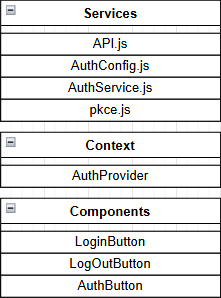
\includegraphics[width=5cm]{./img/fileStructure.png}
\end{center}


Der Login-Prozess wird in drei semantische Kategorien aufgeteilt. An erster Stelle stehen die Komponenten,
die dem Nutzer die Interaktion mit der Authorisierungs-Logik ermöglichen. 
\subsubsection{Components}
Obwohl theoretisch auch eine einzelne Komponente für den Login-Prozess ausreichen würde, wurde der Login/Logout-Button
im Sinne der Übersichtlichkeit gedrittelt. Der Login- sowie Logout-Button sind sind in der Logik bis auf die ausgeführte Methode identisch: \ref{list:loginbutton}

Der Login-Button, welcher aus der Unternehmens-internen React-Bibliothek entnommen wird, ruft bei Interaktion die \texttt{login()}-Methode 
aus dem Authentifizierungs-Kontext auf, welcher im nächsten Abschnitt beschrieben wird.\break
Der gleiche Prozess findet beim Logout-Button statt, nur dass hier die \texttt{logout()}-Methode aufgerufen wird. \ref{list:logoutbutton}

Diese beiden Komponenten werden dann im AuthButton kombiniert, wobei der Auth-Status entscheidet, 
welcher Button angezeigt wird: \ref{list:authbutton}
Für die Entscheidung, welcher Button angezeigt wird, wird zuerst über die \texttt{useAuth()}-Hook\footnote{In JavaScript, speziell in React, ist eine Hook eine Funktion, mit der ein Zugriff auf React-Features wie State oder Lifecycle-Methoden in Funktionskomponenten möglich gemacht wird}
der Authentifizierungs-Kontext abgerufen. Der daraus resultierende Boolean-Wert \texttt{isAuthenticated} gibt an, ob der Nutzer eingeloggt ist oder nicht.
Mit diesem Boolean-Wert wird dann entschieden, ob der Login- oder Logout-Button angezeigt wird. Das geschieht in diesem Fall mithilfe eines ternären Operators,
der den Wert von \texttt{isAuthenticated} überprüft und abhängig vom Wert den entsprechenden Button zurückgibt.\footnote{\url{https://developer.mozilla.org/en-US/docs/Web/JavaScript/Reference/Operators/Conditional_operator}}
\subsubsection{Context}
Der Authentifizierungs-Kontext ist ein zentraler Bestandteil der Authorisierungs-Logik. Er stellt die Methoden \texttt{login()} und \texttt{logout()} 
zur Verfügung, ist aber zusätzlich auch für die Verarbeitung des Callbacks von Cognito zuständig.
Zuerst werden für den Kontext die benötigten Hooks importiert und ein Context-Objekt erstellt: \ref{list:authcontextimports} \ref{list:authcontextvariables}
Daraufhin werden für den Kontext relevante Variablen definiert, die den User, den Authentifizierungsstatus und die Tokens enthalten:
Die \texttt{login()}-Methode generiert einen zufälligen State und einen PKCE-Verifier, speichert diese im Session Storage und 
leitet den Nutzer zur Authentifizierungs-URL weiter: \ref{list:authcontextlogin}
Die \texttt{logout()}-Methode löscht den Session Storage und leitet den Nutzer zur Logout-URL weiter: \ref{list:authcontextlogout}
Die \texttt{handleCallback()}-Methode wird aufgerufen, wenn der Nutzer nach der Authentifizierung zurück zur Anwendung geleitet wird.
Das wird durch die \texttt{useEffect()}-Hook realisiert, die prüft, ob der Nutzer auf der Callback-Route ist und ob ein Code in der URL vorhanden ist. \ref{list:authcontextcallback}
Die \texttt{handleCallback()}-Methode extrahiert den Code und den State aus der URL, vergleicht den State mit dem im Session Storage gespeicherten Wert und tauscht den Code gegen Tokens aus.
Falls der Austausch erfolgreich ist, werden die Tokens im Zustand gespeichert und der Nutzer wird zur Dashboard-Seite weitergeleitet: \ref{list:authcontextcallback2}
Die \texttt{AuthProvider}-Komponente stellt den Authentifizierungs-Kontext für die gesamte Anwendung bereit: \ref{list:authcontextprovider}
Die \texttt{useAuth()}-Hook ermöglicht den Zugriff auf den Authentifizierungs-Kontext in anderen Komponenten der Anwendung.
\subsubsection{Service}    
Der Service-Ordner enthält unterstützende Funktion für die Authorisierung, wie die Generierung des PKCE-Verifiers 
und -Challenges, den Austausch des Codes gegen Tokens und die Erstellung der Authentifizierungs-URL.
Zuerst muss dafür die Konfiguration definiert werden, mit der gearbeitet wird.
\subsubsection{AuthConfig}
Die \texttt{authConfig.js}-Datei enthält die Konfiguration für die Authentifizierung, einschließlich der Endpunkte, Client-ID und Redirect-URI. 
Zusätzlich wird auch die Basis-URL der API definiert, um später API-Anfragen zu ermöglichen:\ref{list:authconfig}
Mit dieser Konfiguration wird nun gearbeitet, um alle weiteren benötigten Daten zu generieren.
\subsubsection{AuthService}
Der AuthService enthält drei Methoden, die für die Authorisierung benötigt werden:
\begin{itemize}
    \item \texttt{buildAuthUrl()}: Diese Methode generiert die Authentifizierungs-URL, die den Nutzer zur Cognito-Anmeldeseite weiterleitet.
    \item \texttt{exchangeCodeForTokens()}: Diese Methode tauscht den erhaltenen Code gegen Tokens aus, die für die Authentifizierung und Autorisierung verwendet werden.
    \item \texttt{refreshTokens()}: Diese Methode aktualisiert die Tokens, wenn sie abgelaufen sind.
\end{itemize}
Die \texttt{buildAuthUrl()}-Methode erstellt die Authentifizierungs-URL, indem sie die Konfiguration und die PKCE-Challenge verwendet: \ref{list:buildAuth}
Die \texttt{exchangeCodeForTokens()}-Methode tauscht bei Rückruf von der Cognito-Authentifizierung den mitgegebenen Code für ein gültiges
Auth-Token. Dieses kann dann verwendet werden, um API-Abfragen durchzuführen: \ref{list:exchangecodefortoken}
Dafür werden zuerst die nötigen Konfigurations-Daten geladen und die Parameter für die URL-Suche definiert. Mit diesen Daten wird dann 
eine Anfrage an den TokenEndpoint gesendet und die Antwort als das Token zurückgegeben, sollten keine Fehler auftreten.
\subsubsection{PKCE}
PKCE(Proof Key for Code Exchange) ist eine Erweiterung des OAuth 2.0-Protokolls, welches zusätzliche Sicherheit für Clients verspricht,
die nicht in der Lage sind, ihre Client-Geheimnisse sicher zu speichern.
Innerhalb dieser Anwendung wird PKCE verwendet, um den Authentifizierungsprozess sicherer zu gestalten. Dies geschieht über zwei Methoden,
\texttt{generateVerifier()} und \texttt{generateChallenge()}, die jeweils den Verifier und die Challenge generieren. \break

Die \texttt{generateVerifier()}-Methode generiert einen zufälligen Verifier, der als Basis für die Challenge dient. Das geschieht, indem 
ein Array von 32 zufälligen Bytes generiert wird, welches dann in einen hexadezimalen String umgewandelt wird: \ref{list:pkceverifier}
Die \texttt{generateChallenge()}-Methode nimmt den Verifier als Eingabe und generiert die Challenge, indem der Verifier in einen SHA-256-Hash umgewandelt wird.
Das Ergebnis wird dann in einen Base64-URL-kodierten String umgewandelt: \ref{list:pkcechallenge}
\subsubsection{API}
Der API-Service ist die Hook \texttt{useApi()}, welche für die Kommunikation mit der Backend-API zuständig ist. 
Sie Kapselt die Methode \texttt{callAPI()} ab, welche den Zugriff auf die Konfigurierte API ermöglicht: \ref{list:callApi}
Die Daten, die aus der \texttt{callApi()}-Methode zurückgegeben werden, können dann in den Komponenten verwendet werden, um die Daten anzuzeigen oder zu verarbeiten.
\subsection{Dynamische Formularlogik und User Interface}
Das User Interface der Anwendung ist in mehrere Komponenten unterteilt, die jeweils für verschiedene Teile der Anwendung zuständig sind:\break
\begin{center}
    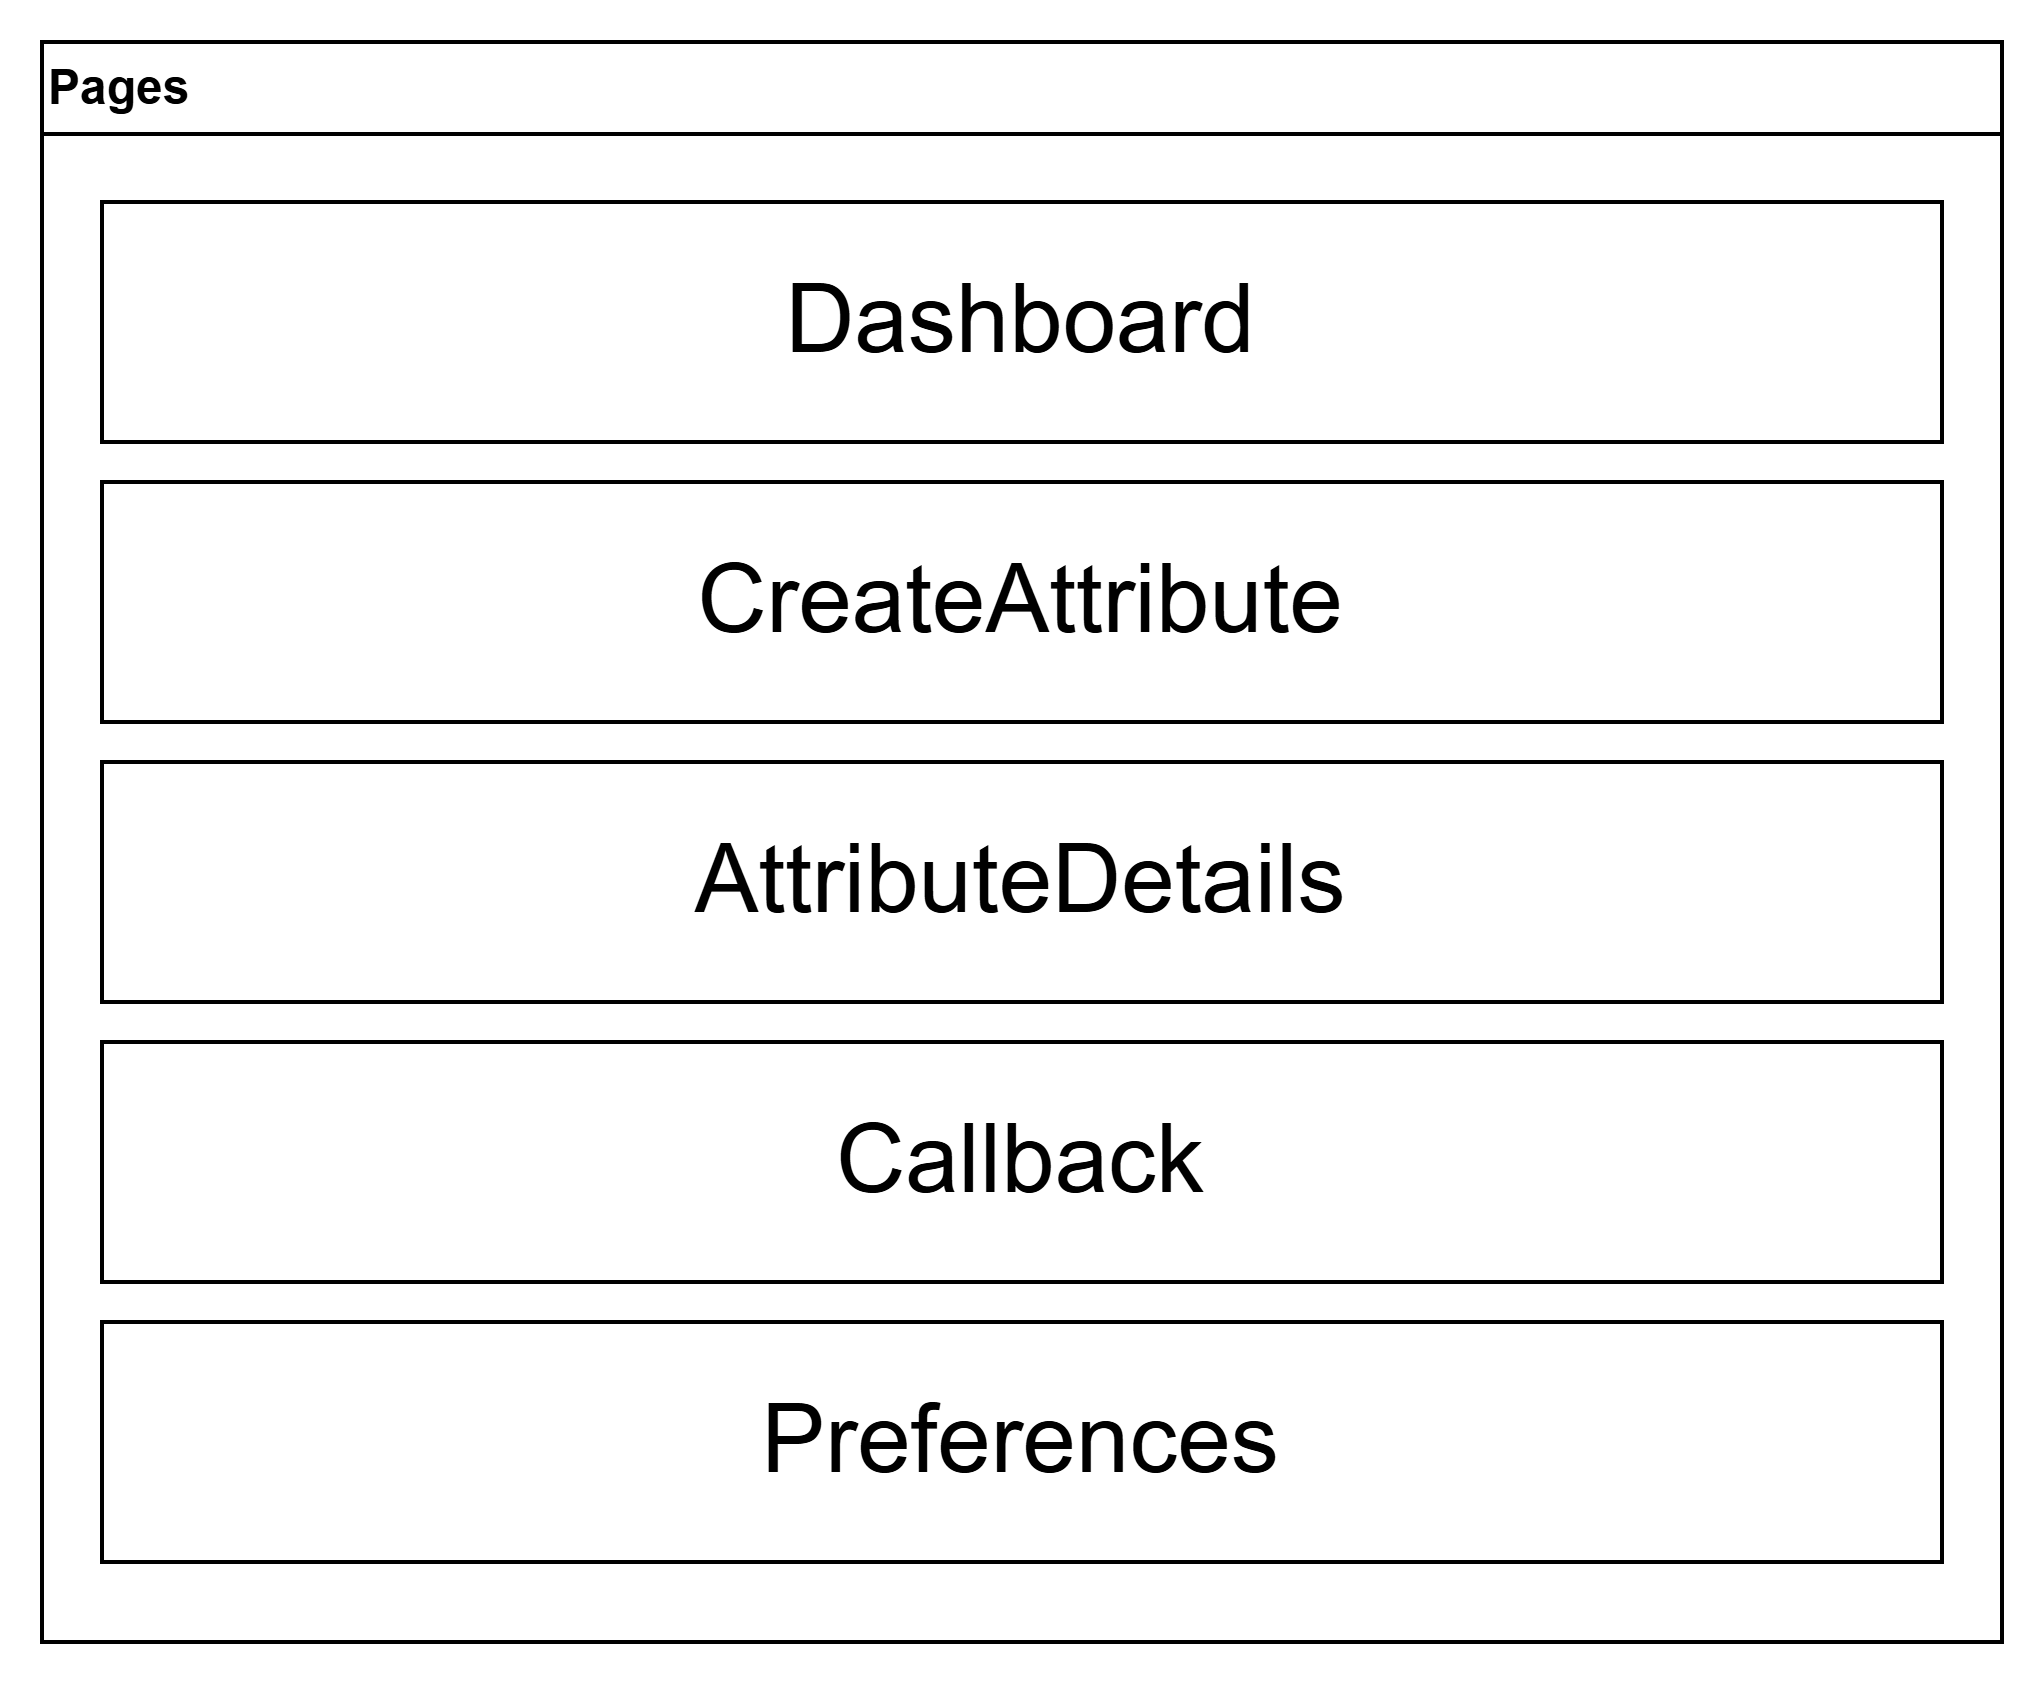
\includegraphics[width=5cm]{./img/dashboardFileStructure.png}
\end{center}
Den Kern der Anwendung bildet die \texttt{Dashboard}-Komponente, welche die Hauptansicht der Anwendung beinhaltet. Von hier aus werden die verscheidenen
Unterseiten aufgerufen (mit Ausnahme der Callback-Seite, die nur für die Authorisierung zuständig ist).
\subsection{Anwendungsbeispiel}
Im Folgenden soll anhand eines konkreten Anwendungsbeispiels die Funktionsweise der Anwendung verdeutlicht werden. Dabei soll gezeigt werden, wie ein Attribut erstellt,
zugeordnet, bearbeitet und gelöscht werden kann. Dadurch soll die Funktionsweise des Systems aus Sicht eines Endnutzers erklärt werden.

\subsubsection{Anlegen eines neuen Attributs}
Um ein neues Attribut anzulegen, navigiert der Nutzer zur \texttt{Attributserstellung}, indem er den entsprechenden Button im Dashboard klickt. 
Daraufhin wird der Nutzer aufgefordert, die erforderlichen Informationen für das Attribut einzugeben. Dabei wird im Hintergrund durch die Anwendung 
die Konformität der Eingaben überprüft, und gegebenenfalls eine Fehlermeldung angezeigt. Durch klicken des \texttt{Next}-Buttons kann der Nutzer dann
die Eingaben bestätigen und die zweite Seite der Attributserstellung aufrufen.
\begin{center}
    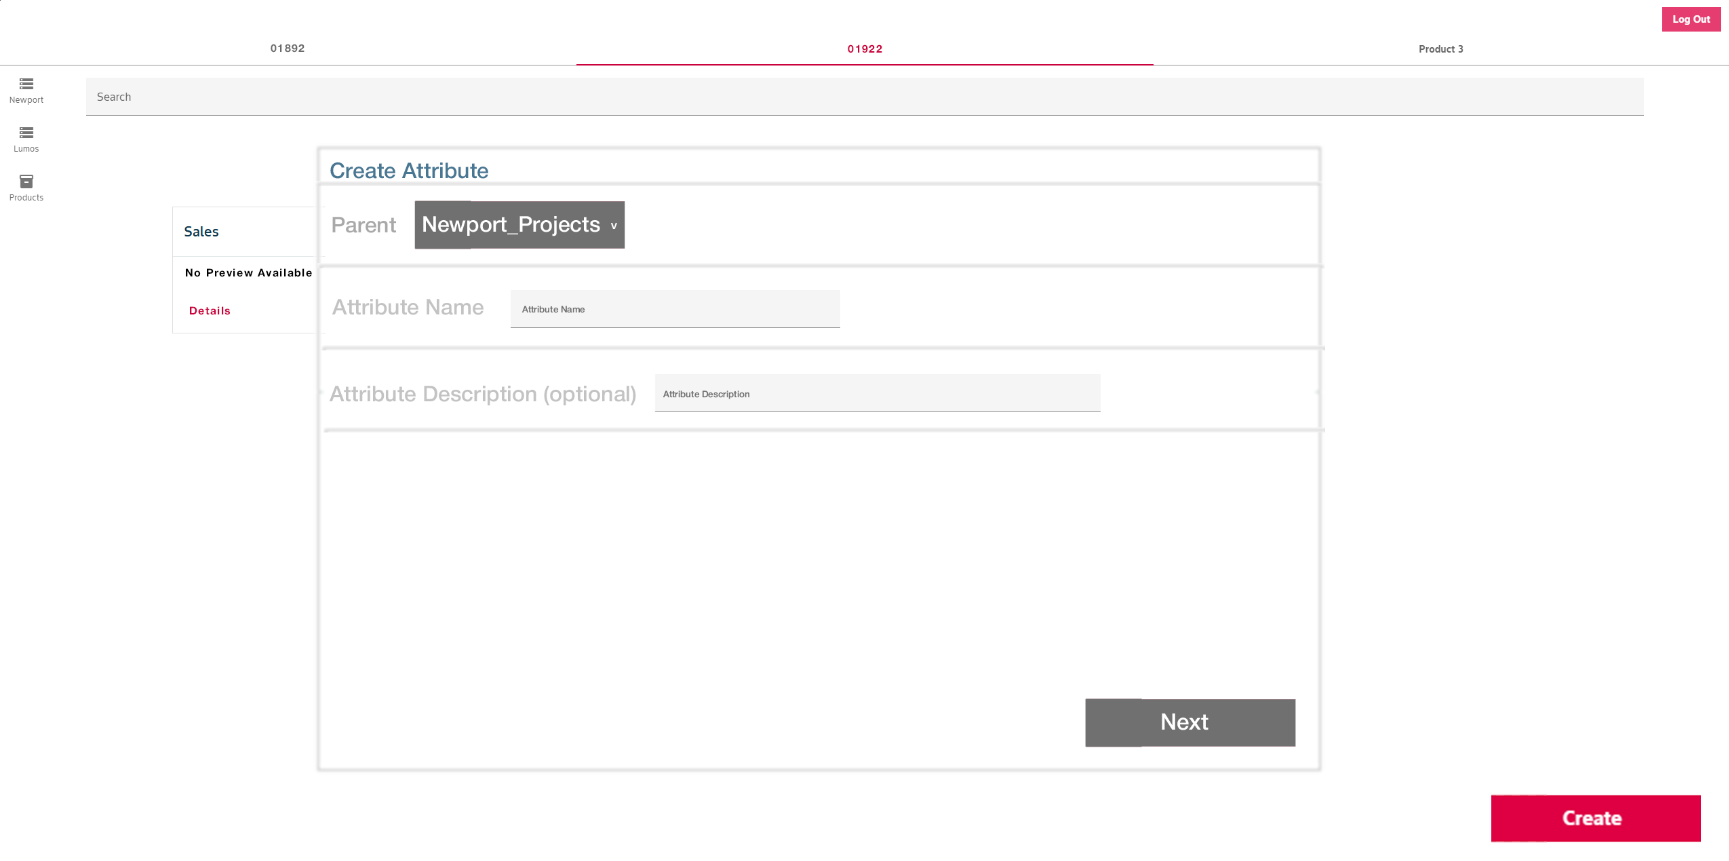
\includegraphics[width=\linewidth]{./img/attributKreation1.png}
\end{center}

Die zweite Seite der Attributserstellung ermöglicht es dem Nutzer, dem Attribut sofort Werte hinzuzufügen. Dafür werden zuerst Informationen über die Art der Werte 
abgefragt, woraufhin der Nutzer die Werte in einer Tabelle eingeben kann. Durch klicken des \texttt{Create}-Buttons kann der Nutzer dann seine Eingaben bestätigen,
und das Attribut wird erstellt. Im Hintergrund wird dafür die API aufgerufen, die das Attribut in der Datenbank anlegt. 

\subsubsection{Bearbeiten eines Werts}
Um einen Wert zu bearbeiten, navigiert der Nutzer zuerst auf die Detailansicht des Attributs, in welchem der Wert enthalten ist. Dort findet er eine Tabelle vor, 
die alle Werte aufführt, und ihm ermöglicht, die Werte zu bearbeiten. Durch klicken des \texttt{Save}-Buttons kann der Nutzer dann seine Änderungen speichern. Im 
Hintergrund wird dafür die API aufgerufen, die den Eintrag in der Datenbank aktualisiert. 
\subsubsection{Löschen eines Attributs}
Um ein Attribut zu löschen, navigiert der Nutzer auf die Detailansicht des Attributs, welches er löschen möchte. Dort findet er einen \texttt{Delete}-Button,
der ihn auffordert, das Löschen zu bestätigen. Nach der Bestätigung wird das Attribut gelöscht, und der Nutzer wird auf die Startseite zurückgeleitet. Im Hintergrund
wird dafür die API aufgerufen, die den Eintrag und alle zugehörigen Referenzen in der Datenbank löscht.
\subsubsection{Zusammenfassung der Attributverwaltung}
Das User Interface ist darauf ausgelegt, dem Nutzer eine einfache und intuitive Möglichkeit zu bieten, Attribute zu erstellen, zu bearbeiten und zu löschen. 
Dafür soll der Nutzer in möglichst wenigen Schritten zu seinem Ziel gelangen, und die Anwendung soll ihn aktiv unterstützen, indem sie im Hintergrund möglichst 
viele Aufgaben übernimmt. Beispielsweise wird die Zugehörigkeit zu einem semantischen Projekt automatisch erkannt, und der Nutzer muss dieses nicht manuell angeben.
\subsection{Herausforderungen und Entscheidungen}

Während der Umsetzung des Frontends sind verschiedene Herausforderungen aufgetreten, die sich nicht nur auf den Code selbst, sondern auch auf Nutzerführung, Fehlerverhalten und Wartbarkeit ausgewirkt haben. Im Folgenden sollen die wichtigsten dieser Punkte - und die Entscheidungen, die daraus resultierten - kurz beschrieben werden.

\subsubsection*{Dynamisches UI ohne Sonderfälle}
Eine der zentralen Fragen war: Wie lässt sich ein Interface bauen, das automatisch auf neue Attribute reagiert, ohne dass man bei jeder kleinen Änderung im Code 
nachbessern muss? Die Lösung bestand darin, Eingabeformulare komplett dynamisch zu generieren - also zur Laufzeit auf Basis der hinterlegten Attribut-Definitionen.  
Das macht den Code insgesamt generischer, aber auch schwerer lesbar. Trotzdem war es die bessere Entscheidung, da so alle Objekte (Formulierungen, Segmente etc.)
 einheitlich behandelt werden können. Anpassungen am Layout einzelner Felder wurden bewusst vermieden, um die Wartbarkeit nicht zu gefährden.

\subsubsection*{Validierung: sofort oder später?}
Ursprünglich war angedacht, die Validierung ausschließlich über das Backend laufen zu lassen - also Fehler erst nach einem Request zurückzumelden. Das führte aber zu 
Frust, weil Nutzer:innen gar nicht wussten, ob ihre Eingaben korrekt sind.  
Deshalb wurde zusätzlich eine einfache Validierung im Frontend umgesetzt: Pflichtfelder, Datentypen und leere Eingaben werden direkt geprüft, bevor überhaupt ein 
Request abgeschickt wird. Dadurch werden Fehler früher abgefangen, ohne dass die API komplett entlastet werden muss.

\subsubsection*{Generik trifft auf Lesbarkeit}
Weil viele Teile des Frontends dynamisch funktionieren müssen, ist der Code an manchen Stellen weniger intuitiv. Zum Beispiel müssen nicht nur Felder, sondern auch 
zugehörige State-Objekte, Event-Handler und API-Requests zur Laufzeit angepasst werden.  
Um das im Griff zu behalten, wurden klare Zuordnungen zwischen Attributtyp und UI-Komponente eingeführt - z. B. dass „Zahl“ immer ein bestimmtes Input-Feld erzeugt. 
Solche Regeln wurden in Hilfsfunktionen ausgelagert, damit die Hauptkomponenten übersichtlich bleiben.

\subsubsection*{Fehlertoleranz bei API-Problemen}
Da das Frontend stark auf die API angewiesen ist, war schnell klar: Wenn eine Anfrage scheitert oder langsam ist, muss das UI trotzdem stabil bleiben.  
Deshalb wurden für alle Requests Lade- und Fehlerzustände eingebaut, die direkt im UI angezeigt werden. Das heißt: Buttons deaktivieren sich automatisch bei 
laufender Anfrage, Fehler werden in Klartext angezeigt - und das System bleibt insgesamt bedienbar, auch wenn das Backend mal nicht reagiert.

\subsection{Fazit zur Frontend-Implementierung}
Im Rahmen des Frontends wurde eine benutzerfreundliche und sichere Anwendung entwickelt, die es Nutzern ermöglicht, Attribute zu erstellen, zu bearbeiten und zu löschen.
Um die Erweiterbarkeit und Wartbarkeit der Anwendung zu gewährleisten, wurde eine modulare Struktur gewählt, durch welche neue Funktionen und Komponenten einfach hinzugefügt
werden können. Die Anwendung ist so konzipiert, dass Nutzer einfach und intuitiv mit ihr interagieren können, während im Hintergrund komplexe Logik und Sicherheitsmaßnahmen
abgearbeitet werden. Dafür wurden folgende Features implementiert:
\begin{itemize}
    \item Dynamische Attributerstellung
    \item Zuweisung von Attributen zu Datenobjekten
    \item Werteingabe und Validierung
    \item Bearbeiten und Löschen von Werten
    \item Dynamisches Rendering von Formularen
    \item API-Kommunikation mit Lade- und Fehlerstatus
    \item Zustandsverwaltung mit React Hooks
    \item Grundlegende Benutzerführung
    \item Selbsterklärende Struktur und Modularität
\end{itemize}

%!TEX root = ../Thesis.tex
\section{Evaluierung}
Im Folgenden soll die Anwendung auf Basis der zuvor definierten Ziele evaluiert werden. Dabei soll zuerst die Einhaltung der funktionalen,
und daraufhin die der nicht-funktionalen Ziele bewertet werden.\footnote{Ich arbeite momentan an einer ordentlichen wissenschaftlichen Evaluierung mit KPIs, das hier ist nur eine erste grobe Einschätzung.}
\subsection{Funktionale Zielerreichung}
Die funktionale Zielerreichung ist anhand der Erfüllung der Must-Have-Anforderungen zu bewerten. Diese sind in der folgenden Tabelle zusammengefasst:
\begin{table}[H]
    \centering
    \caption{Funktionale Zielerreichung}
    \label{tab:funktionaleZielerreichung}
    \begin{tabular}{|p{0.2\textwidth}|p{0.6\textwidth}|p{0.1\textwidth}|}
        \hline
        \textbf{Anforderung} & \textbf{Beschreibung} & \textbf{Erfüllt} \\ \hline
        Anlegen neuer dynamischer Attribute & Nutzer*innen können neue Attribute anlegen, die einem Projektelement zugewiesen werden können. & Ja \\ \hline
        Zuweisung von Attributen zu konkreten Einträgen & Bereits definierte Attribute können spezifischen Datenbankeinträgen zugeordnet und mit Werten befüllt werden. & Ja \\ \hline
        Anzeige und Bearbeitung vorhandener Attribut-Werte & Alle zugewiesenen Attribute mitsamt ihren Werten für ein Projektelement werden angezeigt und sind editierbar. & Ja \\ \hline
        Löschung von Attribut-Zuweisungen & Bestehende Attribut-Wert-Paare können entfernt werden, ohne das globale Attribut zu löschen. & Ja \\ \hline
        Benutzerführung und Eingabeunterstützung & Die Oberfläche bietet verständliche Beschriftungen, Platzhaltertexte und Tooltips zur Unterstützung der Nutzer. & Ja \\ \hline
    \end{tabular}
\end{table}
Von einem funktionalen Standpunkt sind die Ziele vollständig erreicht. Alle definierten Must-Have-Anforderungen sind implementiert und funktionieren wie vorgesehen.
\subsection{Nicht-funktionale Zielerreichung}
Die nicht-funktionale Zielerreichung ist anhand der Response-Time und der Zukunftstauglichkeit der Anwendung zu bewerten. Diese sind in der folgenden Tabelle zusammengefasst:
\begin{table}[H]
    \centering
    \caption{Nicht-funktionale Zielerreichung}
    \label{tab:nichtfunktionaleZielerreichung}
    \begin{tabular}{|p{0.2\textwidth}|p{0.6\textwidth}|p{0.1\textwidth}|}
        \hline
        \textbf{Anforderung} & \textbf{Beschreibung} & \textbf{Erfüllt} \\ \hline
        Performance & Ladezeit für die Anzeige eines Projektelements inklusive dynamischer Felder liegt unter 2000 ms. & Ja \\ \hline
        Skalierbarkeit & Die Lösung ist so ausgelegt, dass sie mit wachsender Datenmenge und Nutzerzahl ohne grundlegende Umstrukturierung betrieben werden kann. & Ja \\ \hline
        Datenintegrität und Validierung & Alle Eingaben werden auf Plausibilität und Formatkonformität geprüft, um konsistente Daten zu gewährleisten. & Ja \\ \hline
        Wartbarkeit & Der Quellcode ist modular strukturiert und dokumentiert, um zukünftige Weiterentwicklungen zu erleichtern. & Ja \\ \hline
    \end{tabular}
\end{table}
Die nicht-funktionalen Ziele sind ebenfalls vollständig erreicht. Die Anwendung reagiert schnell und ist so aufgebaut, dass sie auch bei wachsender Nutzerzahl und Datenmenge performant bleibt. Die Datenintegrität wird durch Validierungen sichergestellt, und der Quellcode ist modular und gut dokumentiert.

%!TEX root = ../Thesis.tex
\section{Fazit}
Im Rahmen dieser Bachelor-Arbeit sollte ein technisches Framework entwickelt werden, mit welchem es möglich ist, benutzerspezifische Informationen 
dynamisch zu bestehenden Datensätzen zu speichern, ohne die zugrunde liegende Datenstruktur anpassen zu müssen.

Im Zentrum stand dabei die Frage, inwieweit diese Flexibilität einen Einschnitt in die Integrität der Daten, die Benutzerfreundlichkeit und Wartbarkeit 
des Systems darstellt. Die Ergebnisse der Arbeit zeigen, dass eine solche Lösung technisch realisierbar und im praktischen Betrieb stabil einsetzbar ist.

Sowohl das Datenmodell als auch das Frontend wurden so konzipiert, dass Erweiterungen möglich sind, ohne dabei bestehende Strukturen verändern zu müssen.
Der modulare Aufbau der Anwendung ermöglicht es, neue Komponenten mit überschaubarem Aufwand zu integrieren.
Besonderer Fokus lag auf einer klaren Trennung zwischen API-Kommunikation, Benutzeroberfläche und der Geschäftslogik - wodurch die Wartbarkeit 
langfristig gesichert wird. 

In der Evaluation konnte gezeigt werden, dass alle funktionalen Kernanforderungen erfüllt wurden. 
Auch unter Last und nicht-idealen Bedingungen (z. B. langsamer Verbindung oder inkorrekter Nutzereingaben) zeigt sich die Anwendung robus und nutzbar.

Trotzdem bleiben weiterhin offene Punkte: Die Durchsatzrate der API ist noch nicht ausreichend, um die prognostizierte maximale Last vollständig zu bewältigen.
Darüber hiknaus ist langfristig ein Rollen- und Rechtesystem erforderlich, um den Schutz sensibler Daten zu gewährleisten.

Insgesamt zeigt diese Arbeit, dass dynamische Erweiterbarkeit und technische Robustheit kein WIderspruch sein müssen, solange Struktur, Validierung und Nutzerführung
in der Architektur von Beginn an berücksichtigt werden.
	
%%%%%%%%%%%%%%%%%%%%%%%%%%%%%%%%%%%%%%%%%%%%%%%%%%%%%%%%%%%%%%%%%%%%%%%

%!TEX root = ../Thesis.tex
\section*{Anhang}
\addcontentsline{toc}{section}{Anhang}
\fancyhead[R]{Anhang}

\anhangsverzeichnis

\anhang{Gesprächsnotizen}

\subanhang{Gespräch mit Werner Müller}

Gespräch mit Werner Müller am 01.01.2013 zum Thema XXX:
\begin{compactitem}
   \item Über das gute Wetter gesprochen
   \item Die Regenwahrscheinlichkeit liegt immer bei ca. 3\%
   \item Das Unternehmen ist total super
   \item Hier könnte eine wichtige Gesprächsnotiz stehen
\end{compactitem}


\anhang{Abbildungen}
\begin{figure}[h]
    \centering
    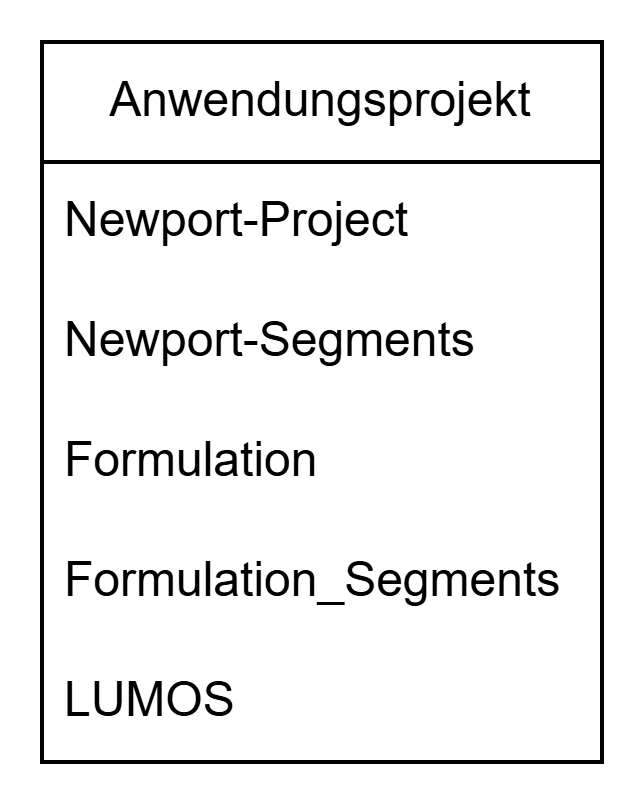
\includegraphics[width=5cm]{./img/projektGrafik.png}
    \caption{projektGrafik}
\end{figure}

\anhang{Listings}
\begin{figure}[H]
    \begin{lstlisting}[caption=JS-Code for the LogIn-Button, breaklines = true, label=list:loginbutton]
        // components/LoginButton.js
        import React from 'react';
        import { useAuth } from '../context/AuthContext';
        import { Button } from '@element/react-components';

        export default function LoginButton() {
            const { login } = useAuth();

            return <Button onClick={login} label="Log In"/>
        }
    \end{lstlisting}
    %\footnoterule{}
    %\footnotesize{Casts have been omitted for the sake of readability}
\end{figure}

\begin{figure}[H]
    \begin{lstlisting}[caption=JS-Code for the LogOut-Button, breaklines = true, label=list:logoutbutton]
        // components/LogoutButton.js
        import React from 'react';
        import { useAuth } from '../context/AuthContext';
        import { Button } from '@element/react-components';

        export default function LogoutButton() {
            const { logout } = useAuth();

            return <Button onClick={logout} label="Log Out"/>
        }
    \end{lstlisting}
    %\footnoterule{}
    %\footnotesize{Casts have been omitted for the sake of readability}
\end{figure}

\begin{figure}[H]
    \begin{lstlisting}[caption=JS-Code for the AuthButton, breaklines = true, label=list:authbutton]
        // components/AuthButton.js
        import React from 'react';
        import { useAuth } from '../context/AuthContext';
        import LoginButton from './LoginButton';
        import LogoutButton from './LogoutButton';

        export default function AuthButton() {
            const { isAuthenticated } = useAuth();

            return isAuthenticated ? <LogoutButton /> : <LoginButton />;
        }
    \end{lstlisting}
    %\footnoterule{}
    %\footnotesize{Casts have been omitted for the sake of readability}
\end{figure}

\begin{figure}[H]
    \begin{lstlisting}[caption=Import und Kontext, breaklines = true, label=list:authcontextimports]
        import React, { createContext, useState, 
        useEffect, useContext } from 'react';
        import { useNavigate, useLocation } from 'react-router-dom';
        import {buildAuthUrl, generateChallenge, generateVerifier, 
        exchangeCodeForTokens} from '../service/authService';
        import authConfig from '../services/authConfig';
        import {generateVerifier, generateChallenge} from '../service/pkce';

        const AuthContext = createContext();
    \end{lstlisting}
\end{figure}

\begin{figure}[H]
    \begin{lstlisting}[caption=Variablen für den Authentifizierungs-Kontext, breaklines = true, label=list:authcontextvariables]
        const [user, setUser] = useState(null);
        const [isAuthenticated, setIsAuthenticated] = useState(false);
        const [tokens, setTokens] = useState(null);
        const navigate = useNavigate();
        const location = useLocation();
    \end{lstlisting}
\end{figure}

\begin{figure}[H]
    \begin{lstlisting}[caption=Login-Methode, breaklines = true, label=list:authcontextlogin]
        async function login() {
            const state = crypto.randomUUID();
            const verifier = generateVerifier();
            const challenge = await generateChallenge(verifier);

            sessionStorage.setItem('oauth_state', state);
            sessionStorage.setItem('pkce_verifier', verifier);
            
            const url = buildAuthUrl({state, code_challenge: challenge});

            window.location.href = url;
        }
\end{lstlisting}
\end{figure}

\begin{figure}[H]
    \begin{lstlisting}[caption=Logout-Methode, breaklines = true, label=list:authcontextlogout]
        function logout() {
            sessionStorage.clear();
            const {logoutEndpoint, clientId, logoutUri} =authConfig;
            window.location.href = `${logoutEndpoint}?client_id=${clientId}&logout_uri=${encodeURIComponent(logoutUri)}`; 
        }
    \end{lstlisting}
\end{figure}

\begin{figure}[H]
    \begin{lstlisting}[caption=Callback-Handling, breaklines = true, label=list:authcontextcallback]
        useEffect(() => {
            if (location.pathname === '/callback' && location.search.includes('code=')) {
                handleCallback();
            }
        }, [location, handleCallback]);
\end{lstlisting}
\end{figure}

\begin{figure}[H]
    \begin{lstlisting}[caption=Callback-Handling, breaklines = true, label=list:authcontextcallback2]
        async function handleCallback() {
            const params = new URLSearchParams(location.search);
            const code = params.get('code');
            const state = params.get('state');
            const saved = sessionStorage.getItem('oauth_state');

            if(!code || !state || state !== saved) {
                return navigate('/', {replace: true});
            }

            try{
                const verifier = sessionStorage.getItem('pkce_verifier');
                const tokenSet = await exchangeCodeForTokens(code, verifier);
                setTokens(tokenSet);

                const [, payload] = tokenSet.id_token.split('.');
                const userInfo = JSON.parse(atob(payload));
                setIsAuthenticated(true);

                sessionStorage.removeItem('pkce_verifier');
                sessionStorage.removeItem('oauth_state');

                navigate('/dashboard', {replace: true});
            } catch (err) {
                console.error('Error during authentication:', err);
                navigate('/', {replace: true});
            }
        }
    \end{lstlisting}
\end{figure}

\begin{figure}[H]
    \begin{lstlisting}[caption=AuthProvider-Komponente, breaklines = true, label=list:authcontextprovider]
        return (
            <AuthContext.Provider 
            value={{ user, isAuthenticated, tokens, login, logout }}>
                {children}
            </AuthContext.Provider>
        );
    }
    export function useAuth() {
        return useContext(AuthContext);
    }
    \end{lstlisting}
\end{figure}

\begin{figure}[H]
    \begin{lstlisting}[caption=AuthConfig, breaklines = true, label=list:authconfig]
        const domain = process.env.REACT_APP_COGNITO_DOMAIN;
        const clientId = process.env.REACT_APP_COGNITO_CLIENT_ID; 
        const redirectUri = process.env.REACT_APP_COGNITO_REDIRECT_URI;
        const logoutUri = process.env.REACT_APP_COGNITO_LOGOUT_URI;
        const apiBaseUrl = process.env.REACT_APP_API_BASE_URL;
        export const authConfig = {
            domain,
            clientId,
            redirectUri,
            logoutUri,
            apiBaseUrl: apiBaseUrl,
            authEndpoint: `https://${domain}/oauth2/authorize`,
            tokenEndpoint: `https://${domain}/oauth2/token`,
            logoutEndpoint: `https://${domain}/logout`,
            responseType: 'code',
            scope: 'openid profile email',
        };
    \end{lstlisting}
\end{figure}

\begin{figure}[H]
    \begin{lstlisting}[caption=Build-Auth Methode, breaklines = true, label=list:buildAuth]
        export function buildAuthUrl({state, code_challenge}) {
            const {
                authorizeEndpoint,
                clientId,
                redirectUri,
                responseType,
                scope
            } = authConfig;
            const params = new URLSearchParams({
                client_id: clientId,
                redirect_uri: redirectUri,
                response_type: responseType,
                scope,
                state,
                code_challenge_method: 'S256',
                code_challenge
            });
            return '${authorizeEndpoint}?{params}';
        }
    \end{lstlisting}
\end{figure}

\begin{figure}[H]
    \begin{lstlisting}[caption=ExchangeCodeForToken Methode, breaklines = true, label=list:exchangecodefortoken]
        export async function exchangeCodeForToken(code, code_verifier){
            const {tokenEndpoint, clientId, redirectUri} = authConfig;

            const params = new URLSearchParams({
                grant_type: 'authorization_code',
                client_id: clientId,
                code,
                redirect_uri: redirectUri,
                code_verifier
            });

            const resp = await fetch(tokenEndpoint, {
                method: 'POST',
                headers: {'Content-Type': 'application/x-www-form-urlencoded' },
                body: params.toString()
            });

            const text = await resp.text();

            if(!resp.ok) throw new Error('Token Exchange failed: $(text)')
            return JSON.parse(text);
        }
    \end{lstlisting}
\end{figure}

\begin{figure}[H]
    \begin{lstlisting}[caption=PKCE-Verifier-Generierung, breaklines = true, label=list:pkceverifier]
        export function generateVerifier() {
            const array = new Uint8Array(32);	
            crypto.getRandomValues(array);
            return Array.from(array, b => ('0'+ b.toString(16)).slice(-2)).join('');
        }
    \end{lstlisting}
\end{figure}

\begin{figure}[H]
    \begin{lstlisting}[caption=PKCE-Challenge-Generierung, breaklines = true, label=list:pkcechallenge]
        export async function generateChallenge(verifier) {
            const encoder = new TextEncoder();
            const data = encoder.encode(verifier);
            const hash = await crypto.subtle.digest('SHA-256', data);
            return btoa(String.fromCharCode(...new Uint8Array(hash)))
                .replace(/\+/g, '-').replace(/\//g, '_').replace(/=+$/, '');
        }
    \end{lstlisting}
\end{figure}

\begin{figure}[H]
    \begin{lstlisting}[caption=PKCE-Challenge-Generierung, breaklines = true, label=list:callApi]
        async function callApi(path, options = {}){
            const url = '${authConfig.apiBaseUrl}${path}';
            const resp = await fetch(url, {
                ...options,
                headers: {
                    'Content-Type': 'application/json',
                    Authorization: 'Bearer ${tokens.access_token}',
                    ...options, headers
                }
            });
            if (!resp.ok) throw 
            new Error('API error ${resp.status}: ${await resp.text()}');
            return resp.json();
        }
    \end{lstlisting}
\end{figure}

\include{chapter/Quellenverzeichnis}


%%%%%%%%%%%%%%%%%%%%%%%%%%%%%%%%%%%%%%%%%%%%%%%%%%%%%%%%%%%%%%%%%%%%%%%

\include{chapter/Ehrenwoertliche_Erklaerung}
 
%%%%%%%%%%%%%%%%%%%%%%%%%%%%%%%%%%%%%%%%%%%%%%%%%%%%%%%%%%%%%%%%%%%%%%%

\printbibliography
\end{document}